\pdfoutput=1
\documentclass[11pt]{amsart}
\usepackage{amsmath,amssymb,amsthm,mathtools}
\usepackage[margin=1.2in]{geometry}
\usepackage{enumitem}
\usepackage{xcolor}
\usepackage{tikz}
\usetikzlibrary{arrows.meta,positioning}
\usepackage[colorlinks=true,linkcolor=blue,citecolor=blue,urlcolor=blue]{hyperref}
\hypersetup{pdfauthor={Bernd Johannes Wuebben},
 pdftitle={Cobordism maps and Atiyah--Floer isomorphisms for framed instanton homology III},
 pdfsubject={Integral comparison of gauge and mixed orientation conventions},
 pdfkeywords={framed instanton homology, Atiyah--Floer conjecture, orientations, excision}}
\setlength{\emergencystretch}{2em}
\raggedbottom
\newtheorem{theorem}{Theorem}[section]
\newtheorem{proposition}[theorem]{Proposition}
\newtheorem{lemma}[theorem]{Lemma}
\newtheorem{corollary}[theorem]{Corollary}
\theoremstyle{definition}
\newtheorem{definition}[theorem]{Definition}
\newtheorem{question}[theorem]{Question}
\newtheorem{convention}[theorem]{Convention}
\theoremstyle{remark}
\newtheorem{remark}[theorem]{Remark}
\theoremstyle{plain}
\newtheorem{thmletter}{Theorem}
\renewcommand{\thethmletter}{\Alph{thmletter}}
\newcommand{\ZZ}{\mathbb Z}
\newcommand{\RR}{\mathbb R}
\newcommand{\SO}{\mathrm{SO}}
\newcommand{\SU}{\mathrm{SU}}
\newcommand{\PD}{\operatorname{PD}}
\newcommand{\ind}{\operatorname{ind}}
\newcommand{\Cone}{\operatorname{Cone}}
\newcommand{\eps}{\varepsilon}
\newcommand{\calib}{\mathrm{cal}}
\newcommand{\CH}{C_{\mathrm H}}
\newcommand{\CJ}{C_J}
\newcommand{\CS}{C_S}
\newcommand{\FH}{F_{\mathrm H}}
\newcommand{\IGJ}{I_J}
\newcommand{\cK}{\mathcal K}
\newcommand{\cM}{\mathcal M}
\newcommand{\orZ}{\operatorname{or}_{\ZZ}}
\title[Atiyah--Floer cobordism maps III]{Cobordism maps and Atiyah--Floer isomorphisms\\
for framed instanton homology III}
\author{Bernd Johannes Wuebben}
\date{26 October 2026.\newline This version: 30 October 2026}
\subjclass[2020]{57K31, 57R58 (primary); 53D40, 58J05 (secondary)}
\keywords{Framed instanton homology, Atiyah--Floer conjecture,
 integral orientations, cobordism maps, excision}
\begin{document}
\begin{abstract}
We construct integral chain homotopy equivalences intertwining the
usual framed instanton cobordism maps in the singular Hopf-link
construction with symplectic cobordism maps oriented by transport
from gauge theory. At common regular small data, the equivalences
are represented by the
Daemi--Fukaya--Lipyanskiy mixed count with a specified coherent
orientation. For connected framed cobordisms, they are natural up
to integral chain homotopy and one overall sign, with an explicit
grading conversion, and extend by geometric changes of
presentation. We also construct equivalences to the normalization
in which attachment of a generating sphere in the surface moduli
space preserves orientation, for every closed connected oriented
three-manifold. Surgery generation gives a finite model built from
one-generator complexes for the three-sphere. Counts through the three-sphere realize
its grading-preserving matrix entries, so an algebraically chosen
normalization becomes a finite integer linear combination of
products of geometric counts. A polynomial in forward and reflected
mixed counts transfers this construction to the symplectic complex.
The proof uses the companion analytic and naturality results and
the stated ordinary surgery and oriented gluing inputs.
Identification with prescribed relative-spin maps and the
nonsingular cap convention remains open.
\end{abstract}
\maketitle
%\setcounter{tocdepth}{1}
%\tableofcontents
%\clearpage

\section{Introduction}

This is the third of three papers on the compatibility of Atiyah--Floer
isomorphisms with cobordism maps. Paper~I~\cite{PaperI} establishes the
comparison over $\mathbb F_2$ and the underlying mixed-equation
analysis. Paper~II~\cite{PaperII} proves integral naturality, up to
one overall sign for each cobordism, with symplectic orientations
transported from the almost-complex gauge convention. The present
paper uses those results to identify the comparison with the usual
singular Hopf-link instanton maps and, at common regular data, with the
Daemi--Fukaya--Lipyanskiy mixed count in a specified coherent
orientation system, and to construct the further
orientation normalization described below. The series thus separates
the analytic comparison, its integral orientation theory, and the
identification and normalization of the resulting maps. The additional
surgery and oriented gluing inputs used here remain explicit.

\subsection{The comparison problem}
The integral form of an Atiyah--Floer comparison depends on the
orientation systems used to define its two chain complexes. Even when
the unsigned moduli spaces coincide, identifying their counts requires
identifying the determinant lines, the action of the gauge group, and
the conventions for quotienting by translation. A comparison of
cobordism maps must in addition control these identifications under
gluing. The allowed ambiguity is a single sign for the whole map.

Paper~II~\cite{PaperII} constructs integral symplectic cobordism maps
by transporting almost-complex gauge orientations through the mixed
equation. Its mixed map intertwines those symplectic maps with the
gauge maps in that convention. Two comparisons are needed to express
this theorem using the usual framed instanton maps and the actual
mixed count of Daemi, Fukaya and Lipyanskiy~\cite{DFL}. The first
compares the usual gauge reference lines with the almost-complex
reference lines on the torus-summed manifold. The second compares
Paper~II's transported orientations with a specified choice in DFL's
coherent orientation construction. We first establish these two comparisons and then construct the
change to DFL's sphere-positive normalization for every object. The analytic constructions and integral naturality theorem of
Papers~I--II remain inputs; their scope is recalled in
Section~\ref{sec:inputs}.

The gauge comparison uses the singular Hopf-link definition of framed
instanton homology in~\cite[Sections~4.3--4.4]{KM} and the excision
cobordism of~\cite[Proposition~5.7]{KM}. The incoming lifting group is
trivial. The outgoing group is the single group specified by the
framing torus in Paper~II. Keeping the subgroup on the cobordism,
rather than only its images at the ends, allows an integral comparison
of coefficients and of the ordinary gluing families.

The orientation choice on the DFL side is specified before defining
any mixed count. In~\cite[Section~2.4]{DFL}, a coherent gauge system
is determined by reference paths and an orientation of a primitive
loop of index four in the framed quotient. We orient this loop and
the reference paths by Paper~II's gauge reference. We call this the
\emph{gauge-calibrated} DFL system. This is one of the choices in the
original construction of~\cite[Sections~2.4 and~4.7]{DFL}. The further
choice discussed in~\cite[Remark~4.76]{DFL}, for which attachment of
a sphere representing the positive generator of the second homotopy
group of the surface moduli space preserves orientation, is a
separate normalization.
We call it the \emph{sphere-positive} system. Theorem~\ref{thm:B} compares the two systems for every closed
connected oriented three-manifold by finite products of actual
counts. The integer coefficients in this construction are chosen
algebraically; the resulting comparison is noncanonical at the
level of its outer maps.

Table~\ref{tab:comparison} separates these conclusions from the
underlying Atiyah--Floer isomorphism. The new assertions concern
the identification and normalization of maps over $\ZZ$, with the
orientation conventions specified here.
\begin{table}[ht]
\caption{The comparison results used in this paper. Each row is
under the hypotheses of the cited construction.}
\label{tab:comparison}
\small
\renewcommand{\arraystretch}{1.15}
\begin{tabular}{@{}p{0.19\textwidth}p{0.76\textwidth}@{}}
\hline
Work & Result and orientation convention \\
\hline
DFL~\cite{DFL} & Integral Atiyah--Floer isomorphism defined by a
mixed count for the admissible gauge and Lagrangian data, including
the framed specialization; coherent orientations
(Theorem~3.29 and Sections~4.7, 7.1). \\
Paper~I~\cite{PaperI} & Geometric cobordism compatibility over
$\mathbb F_2$, with the analytic constructions used by the
integral theory (Theorem~A). \\
Paper~II~\cite{PaperII} & Integral cobordism compatibility up to
one overall sign, with symplectic orientations transported from
the almost-complex gauge convention (Theorem~A). \\
Paper~III & Identification with the usual singular Hopf-link
maps and the gauge-calibrated DFL count (Theorem~\ref{thm:A});
normalization by finite count expressions for every closed
connected oriented three-manifold (Theorem~\ref{thm:B}). \\
\hline
\end{tabular}
\end{table}

\subsection{Objects, maps and statement}
An object is a closed connected oriented three-manifold $M$ with an
oriented ball and the framing data for the torus construction of
Paper~II. A morphism $(W,E,\nu):M_0\to M_1$ consists of a connected
oriented cobordism, a normally framed arc joining the specified balls,
and an $\SO(3)$ bundle trivialized at the ends and along that arc.
All bundle and framing data are part of the morphism. In particular,
a change of an endpoint bundle frame is not identified with the
identity merely because it preserves the underlying manifold.

Write $\CH(M,p)$ for the usual singular Hopf-link instanton complex
at regular data induced by a presentation $p$, with the parity
relabeling of Section~\ref{sec:unit}. Its differential is unchanged
by that relabeling. The usual strict cobordism map is $\FH(W,E,\nu)$.
It uses a homology orientation and the I-orientation prescribed by
the singular construction. For a general permitted relative bundle,
any additionally required I-orientation is retained; its two choices
change the whole map by one sign. We do not impose a liftability
condition on $E$. If $f$ is the parity of this map after the relabeling,
put
\[
 \FH^{\mathrm r}=\FH\eps^f,
 \qquad \eps(x)=(-1)^{|x|}x.
\]
This is the conversion from strict to graded maps used in Paper~II.
It is explained in Section~\ref{sec:algebra} and is part of the
statement, not an unspecified scalar sign.

Let $\CJ(M,p)$, $\CS(M,p)$ and
$N_p:\CJ(M,p)\to\CS(M,p)$ be Paper~II's complexes and mixed map.
A \emph{small presentation} has all the presentation data of
Paper~I, Definition~3.3, including original Heegaard genus at least
one, compatible product collars and metrics, and the prescribed
regularizer bounds. Its primary perturbations lie in Paper~II's
small admissible ball. These conditions are recalled in
Section~\ref{sec:inputs}. For a small decomposition
$d$ of a morphism, $S_d(W,E,\nu)$ denotes the composite of Paper~II's
signed geometric symplectic maps. At objects with zero integral gauge
homology we retain its zero-representative convention, with the
contractions described below.

At common regular data for DFL and Papers~I--II, write
$C_G^{\calib}(p)$, $C_S^{\calib}(p)$ and $N_p^{\calib}$ for the
complexes and the actual DFL mixed count with the gauge-calibrated
orientation choice. These data meet both constructions' hypotheses,
including zero additional gauge-end perturbation; the remaining
conditions are specified in Section~\ref{sec:inputs}.
The active Heegaard genus at such data will be
at least two. The following theorem uses the parity-graded integral
homotopy category $\cK(\ZZ)$; $F\simeq\pm G$ means that one sign
makes the difference null-homotopic over $\ZZ$.

\begin{thmletter}\label{thm:A}
For every small presentation $p$ there is an even integral chain
homotopy equivalence
\[
 \widehat\Psi_p:\CH(M,p)\longrightarrow\CS(M,p)
\]
whose projective homotopy class is independent of the auxiliary
choices and is compatible with geometric changes of presentation.
At common DFL data it is represented by
\begin{equation}\label{eq:actual}
 \Psi_p=B_pN_p^{\calib}U_p,
 \qquad U_p=P_pA_p,
\end{equation}
where $A_p:\CH(M,p)\to\CJ(M,p)$ is the Hopf-link excision
equivalence and
\[
 P_p:\CJ(M,p)\longrightarrow C_G^{\calib}(p),
 \qquad B_p:C_S^{\calib}(p)\longrightarrow\CS(M,p)
\]
are orientation-line chain isomorphisms. These maps are constructed
without using an inverse of a mixed map. Moreover,
\begin{equation}\label{eq:coeff-main}
 B_pN_p^{\calib}P_p=N_p
\end{equation}
as signed chain maps at common data.

For every permitted $(W,E,\nu)$, all small endpoint presentations,
and every small decomposition $d$, one has
\begin{equation}\label{eq:theorem-square}
 \widehat\Psi_{p_1}\FH^{\mathrm r}(W,E,\nu)
 \simeq\pm S_d(W,E,\nu)\widehat\Psi_{p_0}.
\end{equation}
The sign is one sign for the entire map. The assertion includes
arbitrary permitted relative bundles, frame changes, and empty or
acyclic complexes. At an arbitrary small presentation,
$\widehat\Psi_p$ is obtained by geometric transport of an actual
common-data DFL count; no original DFL mixed problem is asserted at
data outside its analytic hypotheses.
\end{thmletter}

On homology the theorem gives a projective natural isomorphism
from the usual framed instanton theory, with the stated convention
conversion, to Paper~II's symplectic theory. The comparison maps at
common data respect the relative mod-four gradings on the DFL and
Paper~II complexes. The full statement for geometric words is made
in the parity-graded category, because Paper~II permits
inhomogeneous representatives of such words. It does not assert
that every such representative is homogeneous modulo four.

The substantial steps are the naturality of the geometric excision
comparison (Section~\ref{sec:excision}) and equality of the signed
mixed counts (Section~\ref{sec:mixed}). Section~\ref{sec:extension}
assembles them using Paper~II's geometric presentation maps and
gives explicit integral homotopies. No numerical computation of a sphere
orientation character is used in this proof.

\subsection{Normalization for every manifold}
Write $C_G^+(p)$, $C_S^+(p)$ and $N_p^+$ for the DFL complexes
and actual mixed count with the sphere-positive system. Reference
paths and their orientations are matched with the calibrated system.
The two systems can have different differentials even though the
matrices of their index-zero mixed counts agree. The problem is
therefore to construct chain equivalences on both sides of that
count, with compatible inverse and mixed homotopies.

We specify the class of maps used in this construction. A
\emph{weighted count expression} is a finite integer linear
combination of composable products of the following maps:
ordinary gauge trajectory, continuation and cobordism counts;
the zero-dimensional counts in the interval, pentagon and cylinder
families of Section~\ref{sec:surgery}; the geometric symplectic
words of Paper~II; and the forward and reflected mixed counts of
Section~\ref{sec:reverse}. Orientation-line identifications,
formal degree labels and weights depending on endpoint relative
grading and parity are allowed. A separately specified product
may have any fixed integer multiplicity. Every physical
intermediate critical set is summed over in full.
Thus an expression counts products of existing zero-dimensional
moduli spaces. This definition does not permit an arbitrary
projection onto a Floer generator or an algebraically selected
mixed inverse as a factor. Integral algebraic homotopies may be
used to verify relations between the resulting maps.

\begin{thmletter}\label{thm:B}
Retain the companion inputs of Section~\ref{sec:inputs} and the
ordinary surgery and oriented gluing inputs of
Section~\ref{sec:surgery-inputs}. Let $M$ be any closed connected
oriented three-manifold with the specified ball and framing data.
At every common regular small presentation $p$ there are even
integral chain homotopy equivalences of relative degree zero,
defined by weighted count expressions,
\[
 u_{X,p}:C_X^{\calib}(p)\longrightarrow C_X^+(p),\qquad
 v_{X,p}:C_X^+(p)\longrightarrow C_X^{\calib}(p),\quad X=G,S.
\]
They are mutually inverse up to integral homotopy and satisfy
\begin{equation}\label{eq:positive-square-main}
 v_{S,p}N_p^+u_{G,p}\simeq N_p^{\calib}.
\end{equation}
The assertion includes nonempty acyclic complexes.

A choice of these maps at each common presentation defines
positive presentation maps by weighted count expressions. They
satisfy projective composition, inverse and word-independence
relations and mixed squares with the actual counts $N_p^+$.
Different choices give equivalent systems in the projective
homotopy category.

For every regular small presentation, geometric transport gives
an even equivalence
\[
 \widehat\Psi_p^+:\CH(M,p)\longrightarrow\CS(M,p),
\]
whose common-data representative is
\begin{equation}\label{eq:positive-common}
 \Psi_p^+=B_pv_{S,p}N_p^+u_{G,p}U_p.
\end{equation}
Its projective homotopy class equals that of $\widehat\Psi_p$ in
Theorem~\ref{thm:A}. In particular it intertwines the usual gauge
and Paper~II symplectic cobordism maps for every permitted relative
bundle and framed morphism, with the convention conversion of
Theorem~\ref{thm:A}.
\end{thmletter}

The theorem constructs a system of positive presentation maps.
It does not identify that system with independently prescribed
positive stabilization or relative-spin counts. The individual
maps $u_{X,p}$ and $v_{X,p}$ depend on choices. Their mixed composite
\eqref{eq:positive-common}, however, has the fixed projective
homotopy class of Theorem~\ref{thm:A}.

\subsection{Proof of the calibrated comparison}
Theorem~\ref{thm:A} has two geometric ingredients. First, the
Hopf-link excision equivalence intertwines the usual singular
cobordism maps and the almost-complex gauge maps, after the stated
grading conversion. Second, the calibrated orientation lines
identify Paper~II's mixed count with the actual DFL count
coefficient by coefficient. Composing these identifications with
Paper~II's naturality homotopies proves the assertion at common
data. Geometric presentation maps then extend it to every small
presentation. This argument requires no normalization of the
index-four loop and no inverse of a mixed count.

\subsection{Normalization by surgery generation}
Reversing the primitive index-four orientation changes the sign
of just one component of the mod-four differential. Abstractly,
any finite free integral complex is isomorphic to the complex
with this sign change: split off its cycles and change signs on
a complement. Such a splitting does not itself give a map defined
by moduli spaces. The main step is to realize enough actual count
expressions that the algebraic choice can be made among them.

Ni's surgery-generation theorem~\cite[Theorem~1.4]{Ni}
gives a finite derivation of $M$ from copies of $S^3$. The ordinary
instanton surgery families turn this derivation into a finite
iterated mapping cone $P$, together with actual count expressions
$i:C_G^{\calib}\to P$, $p:P\to C_G^{\calib}$ and an actual
homotopy $pi\simeq1$. All leaves are labelled copies of the same
fixed one-generator sphere datum. Consequently every row of
$i$ and column of $p$ is a finite sum of count products with a
sphere end. Joining one row and one column by the sphere identity
cylinder realizes a matrix unit in the formal leaf coordinates.
This realizes all grading-preserving matrices before one chooses
a normalizing matrix. A finite integer search, whose termination
follows from the cycle-splitting argument, then gives the required
gauge equivalences.

To pass to the symplectic complex, we use the mixed count at the
reflected presentation with literally paired ordinary ends.
The ordinary index-energy identity shows that this transposed
count and the forward mixed count preserve the same finite
filtration. Their diagonal coefficients are units. A finite
polynomial in the two counts therefore supplies a strict reverse
map. This transfers the gauge normalization to the symplectic
side and gives \eqref{eq:positive-square-main}. Contractibility
treats the acyclic endpoints without extending the reflection
pairing beyond its stated domain.

Sections~\ref{sec:excision}--\ref{sec:extension} prove the
calibrated comparison. Section~\ref{sec:correction} describes
the change of differential and its grading signs.
Sections~\ref{sec:surgery}--\ref{sec:normalization} construct
and normalize the finite gauge model; Section~\ref{sec:reverse}
transfers it through the actual mixed count. The final argument
in Section~\ref{sec:positive-presentation} proves presentation
independence and cobordism compatibility. Only the ordinary gauge
surgery families enter the model construction; no mixed surgery
family is needed. Figure~\ref{fig:dependencies} records the proof
dependencies. In particular, the augmented oriented gluing input
at the reducible cut in Section~\ref{sec:surgery-inputs} remains
an input; the comparison of its two local unit faces is proved
here.

\begin{figure}[ht]
\centering
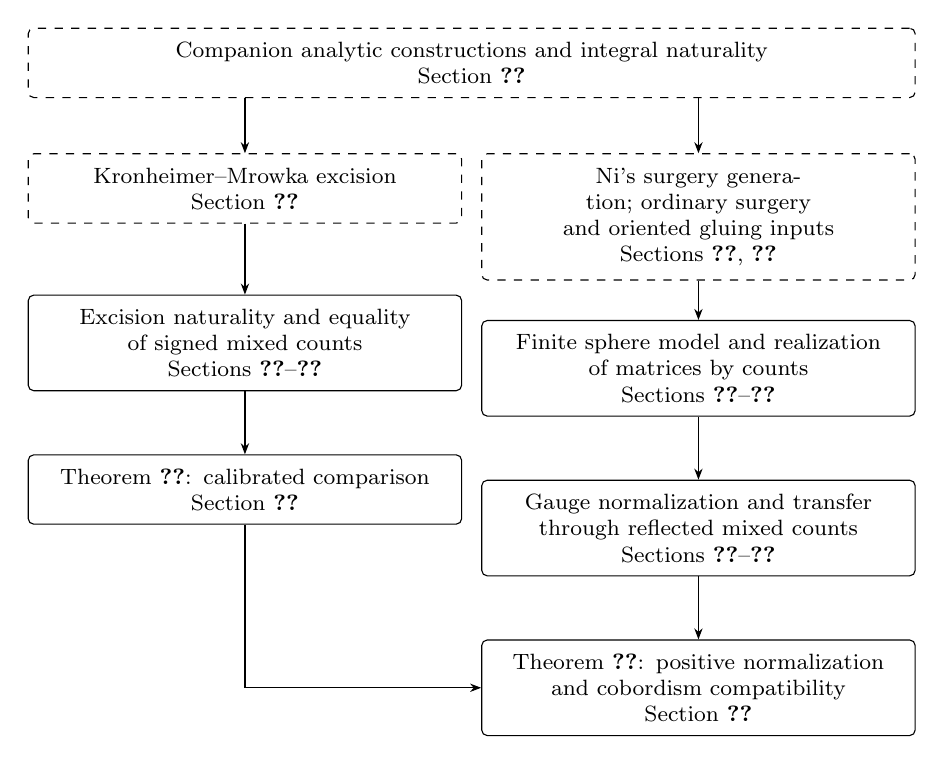
\begin{tikzpicture}[
 box/.style={draw,rounded corners=2pt,align=center,font=\footnotesize,
             text width=0.425\textwidth,inner sep=5pt},
 imported/.style={box,dashed},
 arr/.style={-{Stealth[length=4pt]},thin}]
\node[imported,text width=0.90\textwidth] (comp)
 {Companion analytic constructions and integral naturality\\
  Section~\ref{sec:inputs}};
\node[imported,below=7mm of comp.south west,anchor=north west] (ex)
 {Kronheimer--Mrowka excision\\Section~\ref{sec:excision}};
\node[imported,below=7mm of comp.south east,anchor=north east] (sur)
 {Ni's surgery generation; ordinary surgery\\and oriented gluing inputs\\
  Sections~\ref{sec:surgery-inputs}, \ref{sec:models}};
\node[box,below=9mm of ex] (cal)
 {Excision naturality and equality\\of signed mixed counts\\
  Sections~\ref{sec:excision}--\ref{sec:mixed}};
\node[box,below=5mm of sur] (model)
 {Finite sphere model and realization\\of matrices by counts\\
  Sections~\ref{sec:models}--\ref{sec:normalization}};
\node[box,below=8mm of cal] (a)
 {Theorem~\ref{thm:A}: calibrated comparison\\
  Section~\ref{sec:extension}};
\node[box,below=8mm of model] (norm)
 {Gauge normalization and transfer\\through reflected mixed counts\\
  Sections~\ref{sec:normalization}--\ref{sec:reverse}};
\node[box,below=8mm of norm] (b)
 {Theorem~\ref{thm:B}: positive normalization\\
  and cobordism compatibility\\Section~\ref{sec:positive-presentation}};
\draw[arr] (comp.south -| ex.north) -- (ex.north);
\draw[arr] (comp.south -| sur.north) -- (sur.north);
\draw[arr] (ex) -- (cal);
\draw[arr] (cal) -- (a);
\draw[arr] (sur) -- (model);
\draw[arr] (model) -- (norm);
\draw[arr] (norm) -- (b);
\draw[arr] (a.south) |- (b.west);
\end{tikzpicture}
\caption{Dashed boxes denote imported results and retained inputs;
solid boxes denote arguments of this paper. The companion inputs
are used in both branches, as well as in the final presentation
comparisons.}
\label{fig:dependencies}
\end{figure}

\section{Conventions and imported constructions}\label{sec:inputs}

\subsection{The gauge and symplectic objects}
Form $M^\#=M\#T^3$ along the specified ball. Fix an oriented torus
$T_0$ in the punctured $T^3$ and an odd bundle on $T^3$, so that
$\langle w_2,[T_0]\rangle=1$. Join it to the trivial bundle on $M$.
The framing quotient enlarges the determinant-one gauge group by
\[
 \phi_M=\langle\alpha_M\rangle,
 \qquad \alpha_M=\PD[T_0]\pmod2.
\]
A lifting class is the obstruction to lifting a bundle automorphism
to the determinant-one gauge group. Only this cyclic subgroup is
added; arbitrary classes from $H^1(M;\ZZ/2)$ are not included.
For a morphism insert the punctured torus times an interval in the
framed tube, obtaining $(W^\#,E^\#)$ and its specified subgroup
$\phi_W$. On disconnected cuts the full subgroup on the cobordism
must be retained.

Choose at each object an almost-complex reference $J_0$ on its
cylinder with the fixed product germ near $T_0$. Paper~II uses the
Kronheimer--Mrowka almost-complex orientations, invariant under
bundle automorphisms, and converts the restrictions of cobordism
structures to these object references. A reference conversion is
the determinant-line isomorphism obtained by gluing the operator
between the two references. Its degree can be odd. Paper~II,
Section~4, specifies its position relative to the generator line;
we use its right-placed, graded form for $\IGJ(W)$.

For a Heegaard splitting of genus $g\ge1$ adapted to the fixed
ball, adjoining the torus through its equatorial disk produces two
compression bodies with boundary $\Sigma_h\sqcup T^2$, where
$h=g+1\ge2$. Their boundary collars and product metrics agree on
$\Sigma_h$ and on the torus collar, whose flat metric is fixed for
all presentations. The collar of $\Sigma_h$ meets the gluing sphere
in the product of an interval with the boundary of the equatorial
disk: its lines stay in the punctured torus or in the original
$M$ piece according to their starting point. These are the collar
compatibility conditions of Paper~I, Definition~3.3.
The symplectic space $\cM_h$ is the moduli space of flat connections
on the odd surface bundle, with the lift convention of
\cite[Section~2]{DFL}. Restriction from the compression bodies gives
Lagrangians, moved to $P_0,P_1$ by primary holonomy perturbations.
The primary functions are finite sums of averaged holonomy functions
supported away from the fixed collars. Their trace convention uses
a chosen continuous square root of the determinant holonomy to take
the trace of the $\SU(2)$ part. At regular data $P_0\cap P_1$ is
finite and transverse and corresponds to the gauge critical orbits.

If $L_G(a_x)$ is the real orientation line at a gauge generator,
write $\orZ(L_G(a_x))$ for the free abelian group on its two
orientations, with opposite orientations negatives of one another.
Paper~II defines
\[
 \CS(M,p)=\bigoplus_{x\in P_0\cap P_1}\orZ(L_G(a_x)).
\]
Its differential counts strips oriented by transport through the
mixed equation. A \emph{mixed configuration} is a pair $(A,u)$ consisting of a
connection on the gauge region and a map from the symplectic region,
satisfying the matching, Lagrangian boundary and asymptotic conditions.
The matching condition requires that the boundary connection be flat
and represent the boundary value of $u$. Denote this ambient space,
modulo the specified gauge group, by $\mathfrak B_{\mathrm{mix}}$.
A \emph{mixed solution} is a configuration that also satisfies the
perturbed anti-self-duality and Cauchy--Riemann equations. Determinant
lines below are defined on $\mathfrak B_{\mathrm{mix}}$, and their
transport paths need not consist of solutions. Secondary perturbations
are supported away from the matching boundary and end collars.
The regularizing data include the end perturbation, its mixed
cutoff, secondary data, and the allowed interior almost-complex
changes. Ordinary ends have fixed irreducible nondegenerate limits;
mixed ends retain their varying limiting values as finite-dimensional
stationary coordinates.

The domain defining the comparison is the \emph{special quintuple}
of~\cite[Section~3.1, Figures~1--2]{DFL}. A quintuple records the gauge
four-manifold $X$, its bundle $V$, the symplectic surface $S$, the
surface moduli space, and its Lagrangian boundary conditions. Here
$X$ is assembled from the products of the two compression-body cores
with $\RR$ and the negative half of a four-ended planar domain times
the matching surface. The positive half of that domain is $S$;
the common dividing line is the matching boundary. The two remaining
boundary components of $S$ carry the compression-body Lagrangians.
The resulting domain has one ordinary gauge input, one ordinary
symplectic output, and two mixed ends, one for each compression body.
The matching surface is $\Sigma_h\sqcup T^2$; its moduli-space target
is written as $\cM_h$, since the odd torus factor is a point. This
is the specific mixed domain used in Section~\ref{sec:mixed}.

\subsection{Smallness and the precise companion inputs}
For a primary function $\mathfrak h_i$ on a compression body use
Paper~II's norm, modulo constants,
\begin{align*}
 \|\mathfrak h_i\|_i={}&
 \sup_B\|\nabla_B\mathfrak h_i\|_{L^\infty}
 +\sup_{B\ne B'}
 \frac{\|\nabla_B\mathfrak h_i-\nabla_{B'}\mathfrak h_i\|_{L^2}}
 {\|B-B'\|_{L^2}},\\
 \|\mathfrak h\|={}&\max_i\|\mathfrak h_i\|_i.
\end{align*}
The fixed finite trace family $F_0$ gives embedding coordinates on
the compact unperturbed moduli spaces. In addition, Paper~I fixes
for each splitting a finite family $F_*$ whose universal restriction
map is a submersion at every flat connection of either compression
body. It contains the fixed torus-compression height functions of
Paper~I, Section~10; the two-handle height functions are included
in the enlarged families of the relevant comparisons.
The allowed ambient families $F$ contain both
$F_0$ and $F_*$. The datum lies in Paper~I's neighborhood
$\mathcal U(F)$: a path of primary functions from zero to that datum
keeps the two Lagrangians and their reflections $C^1$-close to the
unperturbed ones, with closeness small relative to those fixed
auxiliary heights. Thus admissibility includes this path condition,
as well as transverse intersections at the chosen endpoint.

A finite family is \emph{separated} if its functions can be written
as affine combinations of averaged sign-sensitive traces on pairwise
disjoint embedded solid tori in the interiors of the compression
bodies. This is a condition on a chosen realization of the family,
not an additional property of a critical point. For primary data
$\mathfrak h$, let $X_i$ be the finite set of restrictions of its gauge
critical points to the interior of the $i$th compression body, modulo
determinant-one gauge transformations. A \emph{split addition} is a
finite sum $g=g_0+g_1$ of cylinder functions whose loops lie in the
respective compression-body interiors and for which $g_i$ vanishes
on a neighborhood of $X_i$. It leaves the common collar unchanged;
if sufficiently small, it also leaves the critical points and Hessians
unchanged. Separatedness
is used for the initial family in the regularization theorem below;
an enlarged ambient family need not remain separated.

The end perturbation is invariant under the framing lift, vanishes
near the critical set, and makes all nonconstant gauge trajectories
of index at most seven in the determinant-one theory regular. Both
it and the secondary data obey the smallness thresholds for the
mixed isomorphism in Paper~I, Theorem~3.8. We call primary data
\emph{DFL-regular} if these gauge trajectories are already regular
with zero additional end perturbation. For fixed splitting
and metric data, Paper~II, Sections~10, 11 and~13, supplies a radius
$r_\chi>0$, independent of enlargements of the finite family, such
that perturbations of norm less than $r_\chi$ retain its required
admissibility and orientation-character properties. Small
presentations include regularizing data making the relevant counts
regular. Small cobordism words are the permitted elementary words
with these data. No assertion below enlarges that smallness domain.

We use the following results of the fixed companion versions
\cite{PaperI,PaperII}.
\begin{enumerate}[label=(\roman*),leftmargin=*]
\item Paper~I, Theorem~3.6 and Appendix~C, supplies arbitrarily
small transverse primary data in a separated finite family, and
arbitrarily small split additions making the gauge data DFL-regular
without changing the metric or losing admissibility. Proposition~3.11
identifies its common mixed problem with DFL's: the extra gauge-end
perturbation is zero, the primary data agree, the secondary
perturbation is invariant under the framing lift, and the special
quintuple, metrics and almost-complex data satisfy the DFL restrictions.
\item Paper~II, Proposition~2.1 and its analytic appendices, supplies
the Fredholm realizations on configuration families, with the primal
matching domain, stationary coordinates and the adjoints on dual
weighted spaces. It includes ordinary gluing and invertible constant mixed pairs.
Proposition~2.2(a) and its proof in Appendix~B supply the following
preparation and shifting statement on the comparison domain. A
compact family in $\mathfrak B_{\mathrm{mix}}$ with fixed asymptotic
labels can first be made stationary beyond a common end cutoff and
then deformed to gauge paths followed by constant mixed pairs $C^c$,
where $c$ is the actual representative over the output label. Both
deformations preserve the matching and Lagrangian conditions and
retain the stationary coordinates. Preparation preserves members
already stationary beyond the cutoff, and shifting keeps members
already of terminal form within that subspace. They are continuous in
configurations and data and coherent with ordinary input gluing.
Its Proposition~5.4 defines the transported orientations
by ordinary gauge orientations and canonically oriented constant
pairs. These are statements on configuration spaces, not only on
solutions.
\item Paper~II gives an even chain isomorphism $N_p$
(Theorem~A and Proposition~6.3)
and, for every morphism and small word, a sign $t_W$ and an integral
homotopy $L_W$ satisfying
\begin{equation}\label{eq:II-square}
 N_1\IGJ(W)-t_WS_d(W)N_0=\delta L_W.
\end{equation}
Its Section~14 constructs the actual geometric continuation,
stabilization, metric, isotopy and decorated-isomorphism maps.
With fixed object references the identity-presentation maps are even,
satisfy mixed squares, and have projective inverse, composition and
word-independence homotopies. General reference conversions retain
their degrees and the sign rules of Section~\ref{sec:algebra}.
\end{enumerate}
These are the analytic existence results and geometric symplectic
maps used in the comparisons below.

\subsection{Strict and graded maps}\label{sec:algebra}
All chain groups are finite free abelian groups with parity grading
and an odd differential. For a homogeneous map $T$ put
\[
 \delta T=d_DT-(-1)^{|T|}Td_C.
\]
Extend this differential componentwise to inhomogeneous maps.
The category $\cK(\ZZ)$ has closed maps modulo $\delta$-boundaries;
composition uses the usual graded Leibniz rule. We further identify
a morphism with its negative when speaking of a projective class.

A strict homogeneous map satisfies $d_DF=Fd_C$, regardless of its
parity $f$. Its graded form is
\begin{equation}\label{eq:right}
 \mathcal R(F)=F\eps_C^f.
\end{equation}
The identities $d\eps=-\eps d$ and
$\eps_DF=(-1)^fF\eps_C$ give
\begin{equation}\label{eq:right-comp}
 \delta\mathcal R(F)=0,
 \qquad \mathcal R(G)\mathcal R(F)=(-1)^{gf}\mathcal R(GF)
\end{equation}
for strict maps of parities $f,g$. Thus the conversion preserves
composition projectively, not necessarily strictly. If
$F_1-F_0=d_DH+Hd_C$ and the endpoint maps have parity $f$, then
\begin{equation}\label{eq:right-homotopy}
 \mathcal R(F_1)-\mathcal R(F_0)=\delta(H\eps_C^f).
\end{equation}
The exponent is the parity of the endpoint maps, whereas $H$ has
parity $f+1$. Throughout, the original differential is retained.

We will also use that an acyclic finite free parity-graded complex
over $\ZZ$ is contractible. Indeed, write $C_i=Z_i\oplus L_i$,
where $Z_i=\ker d_i=\operatorname{im}d_{i+1}$. The quotient by
$Z_i$ is the free subgroup $\operatorname{im}d_i$ of the next
chain group, so this splitting exists, and $d_i:L_i\to Z_{i-1}$
is an isomorphism. The map
\begin{equation}\label{eq:contraction}
 h(z+\ell)=(d|_{L_{i+1}})^{-1}z
\end{equation}
satisfies $dh+hd=1$. Consequently a quasi-isomorphism of finite
free integral complexes is a chain homotopy equivalence, by applying
this construction to its cone. This includes nonempty complexes
with zero homology, without a torsion-freeness hypothesis on the
homology of a general complex.

At a zero-homology object, maps incident to it are null-homotopic.
Paper~II uses zero representatives there; its geometric descriptions
at nonzero-homology objects and this zero convention are both retained.
Zero maps between contractible complexes are homotopy equivalences.
The empty complex requires no critical basepoint or reference path.

\section{The usual gauge maps and Hopf-link excision}\label{sec:excision}

\subsection{The singular realization}
Place the standard Hopf link $H_M$ in the specified ball of $M$,
with its arc $\omega_M$ joining the two components. Before the
parity relabeling below, set
\[
 \CH(M)=C_{\omega_M}(M,H_M;\ZZ).
\]
The gauge group is determinant-one. This is the usual definition
of $I^\sharp(M,\varnothing)$ in~\cite[Section~4.3]{KM}; it is also
$I^\natural(M,U)$ for the small unknot whose meridian is the other
Hopf component. Its reference torsors are those of
\cite[Section~4.4]{KM}. The incoming reference is the preferred
reducible singular connection of that construction.

Transporting the Hopf link through the framed tube of $W$ gives
two oriented annuli $S_H$. For any permitted relative bundle $E$,
retain it outside that tube and perform the singular replacement
inside, using its specified trivialization. Denote the resulting
bundle data by $P_H$. The map $\FH(W)$ is the usual count for
$(W,S_H,P_H)$. For the untwisted bundle, the oriented annuli $S_H$
make the I-orientation equivalent to a homology orientation, as
described after Definition~4.3 and in equation~(26)
of~\cite{KM}. For a general fixed bundle, its I-orientations form
a two-element torsor~\cite[Definition~3.9]{KM}. The determinant
factorization there compares all endpoint generators and relative
classes; changing the I-orientation multiplies every coefficient by
the same sign. We use the usual homology and lift data when they
specify this element, and otherwise retain this single projective
choice.

\begin{proposition}\label{prop:gauge}
There are geometric even integral chain homotopy equivalences
$A_p:\CH(M,p)\to\CJ(M,p)$, with the parity convention of
Section~\ref{sec:unit}, and, for every permitted morphism, a sign
$s_W$ and an integral homotopy $G_W$ such that
\begin{equation}\label{eq:gauge-square}
 A_1\FH^{\mathrm r}(W)-s_W\IGJ(W)A_0=\delta G_W.
\end{equation}
Their construction uses singular excision and ordinary reference
conversions and is independent of mixed maps.
\end{proposition}

\subsection{The excision subgroup and its coefficients}
Apply~\cite[Proposition~5.7]{KM} to the small unknot $U$. Cutting
the two tori around the Hopf components and interchanging meridians
and longitudes gives a cobordism $X_M$ with outgoing components
$(S^3,H)$ and $M\#T^3$. To identify the latter marking, recall that
the complement of a coordinate circle in $T^3$ is
$S^1\times(T^2\setminus\operatorname{int}D^2)$. Under the exchange,
the disk bounded by the zero longitude of the unknot fills the
boundary circle of the punctured torus. The remaining circle is the
$S^1$ factor. The original $M$ lies outside the ball. Its framing
fixes the longitude and hence the required marked torus summand.

The incoming cutting tori are separating, so their dual classes
vanish. The incoming lifting subgroup is zero. The outgoing sphere
also has trivial subgroup, and the outgoing torus-summed component
has precisely $\phi_M$. On $X_M$ we use the actual subgroup $H_X$
of~\cite[Theorem~5.6]{KM}, generated by the duals of the four edge
hypersurfaces $T\times[0,1]$ in its local product $T\times U$, where
$U$ is the excision surface with corners.

Here $H_X\cong\ZZ/2$ and restriction $H_X\to\phi_M$ is an
isomorphism. Indeed, the local surface $U$ is a disk with four
attaching edges. The exterior has three components; two edges attach
to the middle Hopf exterior, and the remaining edges to the two
solid-torus components. The incidence graph therefore has four
vertices and four edges, with one cycle. Each prescribed dual class
restricts to zero on the local piece and on each exterior piece.
It belongs to the degree-zero Mayer--Vietoris contribution, which is
the one-dimensional cycle space of this graph. The outgoing transverse
circle detects its nonzero element. Thus the prescribed subgroup
has no kernel on restriction to the outgoing end. Additional
cohomology of $M$ is not part of this subgroup.

The freeness needed for the quotient is the strengthened
\emph{$\phi$-non-integral condition} of~\cite[Definition~5.1]{KM}.
It holds: $T_0$ is odd for the bundle and
\[
 \alpha_M|_{T_0}=\PD[T_0]|_{T_0}=0
\]
because its normal line is trivial. On the Hopf component the group
is trivial and the standard torus is non-integral. Fixing a
representative of an outgoing critical orbit therefore selects
exactly one representative in every $H_X$-orbit of solutions. This
remains true when the action permutes relative configuration classes:
restriction is injective and surjective on the prescribed group.
The coefficient dictionary uses this bijection, not division by the
order of the group.

Use the almost-complex orientations of~\cite[Sections~5.1 and~5.3]{KM} on
$X_M$, with a product structure on $T\times U$ and complex cutting
tori. The outgoing germ can be chosen to be Paper~II's germ near
$T_0$. The excision count is a strict chain map
\begin{equation}\label{eq:excision-count}
 e_M:C_{\mathrm{Hopf}}^{J_-}(M)\longrightarrow
 V\otimes C_G^{J_+}(M\#T^3),
\end{equation}
where $V=C_\omega(S^3,H)$ has one nondegenerate generator and zero
differential~\cite[Proposition~4.1]{KM}. By the integral excision
theorem~\cite[Theorem~5.6]{KM}, its homology map is an isomorphism.
The rank-one free factor entails neither an eigenspace projection
nor a K\"unneth assertion for two groups with torsion.

\subsection{Reference lines}
Compare the usual singular reference torsor at the incoming end
with the $J_-$ torsor by determinant gluing. There is no incoming
lifting quotient. Choosing an orientation of the single reference
comparison line determines its transport to every generator. The
trajectory factor in the gluing is the same on both sides; ordinary
instanton and monopole addition have the common conventions of
\cite[Sections~3.8 and~4.4]{KM}. This gives a strict reference
isomorphism
\[
 P_M^{\mathrm H}:\CH(M)\longrightarrow C_{\mathrm{Hopf}}^{J_-}(M).
\]
The trivial-subgroup case of~\cite[Section~5.1, p.~154]{KM} identifies
this construction with the usual reference comparison. In a
cobordism the two reference conventions factor the same determinant
line into endpoint factors and one I-orientation torsor. The
remaining sign therefore belongs to the whole map, not separately
to its generators or relative classes.

At the outgoing end use the strict form of Paper~II's reference
conversion
\[
 T_M:C_G^{J_+}(M\#T^3)\longrightarrow\CJ(M).
\]
Both structures have the fixed torus germ. Their difference class
restricts trivially to $T_0$, so the conversion has trivial character
on $\phi_M$, by Paper~II, Proposition~4.2. It consequently descends
to the required quotient. This is the almost-complex conversion of that proposition.

Changing the chosen structures on the excision cobordism changes
the map, after these reference conversions, by a single sign and
an ordinary data homotopy. To see the sign assertion, compare the
two complex orientations on a fixed-end configuration space. Their
ratio is locally constant and is invariant under bundle
automorphisms. The incoming subgroup is zero; the outgoing
conversion has trivial character. Reference gluing and the common
addition conventions compare all endpoint and relative classes,
leaving the one I-orientation choice. This is the determinant
factorization used for Paper~II's gauge functor, applied to these
specified singular and nonsingular ends.

\subsection{The unit factor and the grading}\label{sec:unit}
Fix a complex reference on the Hopf factor and let $v$ be its
generator of parity $\tau$. In the left tensor convention of
\eqref{eq:excision-count},
\[
 d(v\otimes x)=(-1)^\tau v\otimes d_Cx.
\]
The strict contraction is
\begin{equation}\label{eq:unit}
 r_V(v\otimes x)=\eps_C^\tau x.
\end{equation}
It has parity $\tau$, commutes strictly with the differential,
and has inverse $x\mapsto v\otimes\eps_C^\tau x$. For a strict
homogeneous $F$ of parity $f$, the same left tensor convention gives
$(1_V\otimes F)(v\otimes x)=(-1)^{\tau f}v\otimes Fx$. Hence
\begin{equation}\label{eq:unit-naturality}
 r_V(1_V\otimes F)=Fr_V.
\end{equation}
The tensor sign cancels the sign in
$\eps_D^\tau F=(-1)^{\tau f}F\eps_C^\tau$, although the
contraction itself may have generator-dependent signs. Changing
$v$ to $-v$ changes the contraction by one sign.

If the excision induces a Hopf reference of parity $\tau'$,
its strict conversion to the fixed one includes
$\eps_C^{\tau-\tau'}$ on the other tensor factor. Composition with
\eqref{eq:unit} gives $\eps_C^{\tau'}$, up to the chosen sign of
the unit reference. This retains the grading operator when the
free-end structure changes; it does not require prescribing an
arbitrary Hopf plane field at both ends.

In strict conventions define
\begin{equation}\label{eq:A}
 A_M=T_Mr_Ve_MP_M^{\mathrm H}.
\end{equation}
Let $a_M\in\ZZ/2$ be its degree, computed by adding the Fredholm
shifts of these four factors. The relative grading in
\cite[Proposition~5.7]{KM} makes the excision shift independent of
the generators; the reference shifts are fixed per object. The
same definition uses reference operators if a critical set is
empty and does not depend on a nonzero matrix coefficient.
On the source relabel parity by
\begin{equation}\label{eq:parity-relabel}
 |x|_{\mathrm H,new}=|x|_{\mathrm H}+a_M.
\end{equation}
Keep its differential unchanged. The strict map \eqref{eq:A} is
now even and closed. A usual strict map of old parity $f$ has new
parity $f+a_{M_1}-a_{M_0}$ and is converted by
\eqref{eq:right} with that new parity. Index additivity for the
cobordism diagram below identifies it with the parity of the
corresponding torus map. Applying the same index identity to
continuation cylinders shows that $a_M$ is independent of regular
end data. This conclusion does not require a nonzero continuation
coefficient. It is a parity transfer, with the usual grading
recoverable by \eqref{eq:parity-relabel}; it is not an identification
of every absolute grading normalization.

Excision and the rank-one factor make $A_M$ a quasi-isomorphism.
For completeness its integral inverse homotopies can be obtained
from \eqref{eq:contraction}. With cone differential
\[
 D=\begin{pmatrix}d_J&A_M\\0&-d_H\end{pmatrix}
\]
and contraction $h=\left(\begin{smallmatrix}h_J&t\\B&h_H\end{smallmatrix}\right)$,
the equation $Dh+hD=1$ gives
\[
 d_HB=Bd_J,\qquad
 A_MB=1-d_Jh_J-h_Jd_J,\qquad
 BA_M=1+d_Hh_H+h_Hd_H.
\]
This algebra verifies equivalence of the already defined geometric
map. No splitting is used to define $A_M$ or its naturality.

\subsection{The cobordism diagram and the chain homotopy}
The framed tube is $[0,1]\times B^3$ with its given end
identifications. Move the local excision through this tube. Sliding
the surface-with-corners factor in $T\times U$ gives an
identification, relative to the outer ends, of singular cobordisms
with bundle data:
\begin{equation}\label{eq:slide}
 X_{M_1}\circ(W,S_H,P_H)
 \cong\bigl(([0,1]\times(S^3,H))\sqcup(W^\#,E^\#)\bigr)\circ X_{M_0}.
\end{equation}
It is the identity outside the tube and carries the four actual
edge hypersurfaces to the corresponding hypersurfaces. In
particular it preserves the prescribed subgroup, not just its
endpoint images. The relative bundle outside the tube is unchanged.
A frame-change morphism uses its own tube and endpoint
identifications in this construction.

For composition, the left cut in \eqref{eq:slide} is connected.
On the right it is $S^3\sqcup(M_0\#T^3)$. The degree-zero
Mayer--Vietoris map is
\[
 H^0(X_{M_0};\ZZ/2)\oplus
 H^0(([0,1]\times S^3)\sqcup W^\#;\ZZ/2)
 \longrightarrow H^0(S^3\sqcup(M_0\#T^3);\ZZ/2),
\]
with coordinate expression $(a,b,c)\mapsto(a-b,a-c)$. It is
surjective. Thus neither cut supplies an additional connecting
class. The restrictions of the common subgroup are exactly $H_X$,
$\phi_W$, and zero on the Hopf product component. This verifies
the subgroup hypothesis for the disconnected composition in
\cite[Proposition~5.4]{KM} and excludes an extra multiplicity.

Choose a common almost-complex structure for \eqref{eq:slide},
product near its cutting tori and with complex singular annuli.
One may first choose it in the framed tube. In the local Hopf
model a nonzero vector field is tangent to the cores and normal
to the two oppositely oriented cutting tori; in the middle
$T^2\times[0,1]$ it is the interval direction. Extending across
the solid tori interpolates to the chosen core directions. This
gives the local complex structure and its product extension over
the excision piece. Extend the tube germ over $W$, leaving the
outer ends free. The primary obstruction is $W_3(W)=0$ for an
oriented four-manifold; the tube is contractible, and the remaining
obstruction lies in $H^4(W,\mathrm{tube};\ZZ)=0$, since $W$ is
connected with nonempty boundary. Adjust collars to be invariant
at the outer ends. After excision the resulting germ on $W^\#$
is the permitted torus germ. Fixed object references are restored
by the conversions already specified.

There are three ordinary metric families: stretch the left cut,
join the two finite metrics on the common composite, and reverse
the stretch at the right cut. Their endpoints give
$e_{M_1}\FH(W)$ and $(1_V\otimes F_J(W))e_{M_0}$ in the induced
complex conventions. The parameterized constructions are those of
\cite[Section~3.9, following Proposition~3.10]{KM}, with the enlarged
subgroups from its Section~5.1. Two details of this application
are useful. First, the lifting action is free. Choose perturbation
variations in separated neighborhoods of an orbit and translate
them equivariantly. On one representative the available variations
are the original local variations, so they still give surjectivity.
This is the invariant-family argument; averaging an arbitrary
regular perturbation would not by itself prove regularity.
Second, the disconnected cut has two neck parameters. At a rigid
broken solution, regular gluing gives a product chart in the two
large lengths. Restrict this chart to equal lengths. It supplies
the one-parameter end used here. The invertible end operators give
the direct sum of the two end parametrices; the subgroup calculation
above leaves no stabilizer multiplicity. Interior family
perturbations may be chosen relative to these regular ends.

The low-dimensional compactness and gluing statements of
\cite[Sections~3.8--3.9 and~5.1]{KM} apply. In dimensions zero
and one the boundaries are metric endpoints and ordinary Floer
breaking; instanton and monopole bubbling have higher codimension.
Orient the one I-orientation torsor throughout the concatenated
families. In the fiber-first parameter convention the signed
parameter count $H_W$ satisfies the strict relation
$m_1-m_0=dH_W+H_Wd$. Insert the reference conversions and unit
contraction. Equation~\eqref{eq:unit-naturality} introduces no sign;
the comparison of I-orientations introduces only a constant sign. Convert to the
fixed representatives in \eqref{eq:A} and then use
\eqref{eq:right-homotopy}. With the new endpoint-map parity $f$, the
graded homotopy is $G_W=H_W\eps_{\mathrm H,new}^{f}$, including
these fixed conversions. This proves \eqref{eq:gauge-square} and
Proposition~\ref{prop:gauge}.

The same argument for ordinary continuation cylinders makes the
construction at every regular end datum natural. Consequently
$A_p$ is available for arbitrary small presentations, independently
of the additional conditions needed for a common DFL count.

\section{Identification of the signed DFL count}\label{sec:mixed}

\subsection{Choice of the coherent system}
Fix common regular data as in Section~\ref{sec:inputs}, of active
genus $h\ge2$. Suppose first that the critical set is nonempty.
In the determinant-one cover, a primitive framed path joins a
base critical point $a_*$ to its other framed lift and has index
four modulo eight. Its image in the framed quotient is the
primitive index-four loop. DFL, Section~2.4, orients this path
and chooses oriented reference paths from the other generators
to $a_*$. Path gluing and ordinary instanton addition extend the
system. We choose both the primitive orientation and reference
orientations from $J_0$ before applying Sections~4.4 and~4.7 of that
source. We also fix the translation direction specified in
Section~\ref{subsec:terminal-transport}.

The resulting $N^{\calib}$ counts DFL's mixed solutions with
DFL's determinant transport from gauge paths and constant mixed
pairs. Its symplectic orientations are the ones obtained in that
construction. This specifies an orientation system independently
of the value or inverse of any mixed map.

Choose relative mod-four representatives $j(a)\in\{0,1,2,3\}$
with $j(a_*)=0$, and reference paths of index $j(a)$, inserting
primitive loops when necessary. The corresponding gauge and
symplectic degrees agree by~\cite[Proposition~2.54]{DFL}. Setting
this origin does not change determinant-line parity: the constant
difference between the parity and $j$ is retained on both sides.
The reference-path bases and the symplectic bases induced by
constant mixed pairs give even diagonal orientation-line maps
\begin{equation}\label{eq:PB}
 P_p:\CJ(p)\longrightarrow C_G^{\calib}(p),\qquad
 B_p:C_S^{\calib}(p)\longrightarrow\CS(p).
\end{equation}
They are initially identifications of chain groups; their
compatibility with the differentials is proved below.

\begin{proposition}\label{prop:mixed}
The maps \eqref{eq:PB} are chain isomorphisms and satisfy
$B_pN_p^{\calib}P_p=N_p$. This is equality of all signed mixed
coefficients, including off-diagonal coefficients. It uses no
comparison with the sphere-positive normalization.
\end{proposition}

\subsection{A common Fredholm realization}
We first identify operators on the configuration space, because
the orientation constructions transport along nonsolutions.
In Paper~I's common-data coordinates $(t,r)=(\theta,s)$ and
$J_D=-J$, the equations agree. Order the target as Coulomb,
anti-self-dual, and strip rows, as in~\cite[(3.16)]{DFL}.
There is a row convention to check. If $\mathcal J$ is the strip
structure in DFL coordinates, write
\[
 F(u)=\partial_su+\mathcal J(u)\partial_\theta u,
 \qquad Q(u)=\partial_\theta u-\mathcal J(u)\partial_su
             =-\mathcal J(u)F(u).
\]
Differentiation gives
\begin{equation}\label{eq:row}
 D_Q\xi=-\mathcal J D_F\xi-(\nabla_\xi\mathcal J)F(u).
\end{equation}
The second term vanishes at solutions, but cannot be dropped
along a shifting path. Use $Q$ as the common row. After the
permitted preparation of reference configurations to stationary
ones outside a compact set, the correction is a compactly
supported zeroth-order operator. Rellich compactness makes it
compact from the first Sobolev domain to the target. Its action
on stationary coordinates has finite rank. Equivalently, before
truncation, compact-core Rellich and the vanishing tail give the
same conclusion. Scalar interpolation of this correction is a
Fredholm homotopy with unchanged asymptotic operators.

The coordinate pullback identifies the other rows and the primal
matching condition. Ordinary ends are unweighted; at mixed ends
use one common sufficiently small positive weight, with the
stationary coordinates and the same cutoff extensions separated
from the decaying part. These are the spaces in
\cite[Definitions~3.8--3.9]{DFL} and Paper~I's common-data
construction. Paper~II's realized operators and formal adjoints
use precisely these matching domains and dual weights. The
bounded target isomorphism in \eqref{eq:row} transports the adjoint
boundary condition; the zeroth-order correction leaves the
principal boundary pairing unchanged. No spectral wall is crossed.

The target isomorphism and Fredholm homotopy identify determinant
lines on the common space. They also identify ordinary determinant
gluing: the section pullbacks conjugate the pregluing maps, and
the stabilized corrected kernel maps are homotopic through
isomorphisms for sufficiently long necks. At an invertible
operator the determinant line has its canonical orientation.
The target isomorphism preserves it, and the correction in
\eqref{eq:row} is zero at a constant reference pair. Thus the
comparison preserves the terminal constant calibration. The
coordinate notation $J_D=-J$ alone introduces no further
complex-conjugation orientation operation.

\subsection{Transport from a common terminal configuration}
\label{subsec:terminal-transport}
The gauge orientation systems agree on each reference path, on
the primitive framed path, and on ordinary instanton addition.
The path classification and extension rule of
\cite[Section~2.4, the classification preceding (2.48) and the
gluing map (2.55)]{DFL} therefore make them agree
on every gauge path class. Here the quotient adds exactly the
single framing class, as specified above; no further lifting
class requires a separate comparison.

For any mixed configuration use one finite shifting path in the
common special-quintuple configuration space. The relative
preparation and shifting results of Paper~II keep the matching
condition, Lagrangian condition, and stationary coordinates, even
when the limiting mixed value moves. They end at a gauge path
followed by an invertible constant mixed pair $C^c$, for the
representative $c$ actually reached. A finite path suffices; the
orientation comparison requires no limiting infinite translation.
Choose the shift beyond the compact support and dependence of
the secondary perturbation. Compare the terminal constant
operator to its zero-secondary reference through the same small
perturbation path. This path stays invertible by Paper~II,
Proposition~2.1(b), and preserves the canonical orientation.

At this terminal configuration both determinant constructions
use the same ordered gauge factor and the same canonical constant
factor. If $c$ is the other framed lift, use the actual bundle
action on these operators. Conjugation preserves the canonical
orientation of the invertible constant factor, and the calibrated
gauge system accounts for the trajectory factor. Replacing that
action by an arbitrarily declared positive identification would
not be sufficient.

The ratio of the two orientations along the common finite path
is continuous and takes values in $\{1,-1\}$. It is $+1$ at the
terminal configuration, hence at the original one. This proves
the determinant comparison for every mixed component. The
relative shifting statements in the two constructions ensure
independence of the chosen preparation and shift. Alternatively,
one may compare both on the single common path just described;
their individually defined orientations already have that
independence.

For strips glue a constant pair at the input and cancel its
canonically oriented factor. This proves agreement of strip
orientations. We use DFL's fiber-first convention for the quotient
by translation~\cite[p.~17]{DFL}. In both constructions we choose
the positive translation vector to be $\partial_su$ in DFL
coordinates, equivalently $\partial_ru$ in the original coordinates,
in agreement with Paper~II's convention. This choice of direction
is part of our gauge-calibrated system. Gauge trajectories use
the same increasing cylindrical coordinate. Therefore the rigid
trajectory and strip counts give the same differentials under
\eqref{eq:PB}. The isolated mixed counts give exactly
\eqref{eq:coeff-main}, proving Proposition~\ref{prop:mixed}.

Changing a reference-path orientation changes the corresponding
gauge and symplectic bases together. With $P_p$ and $B_p$ changed
accordingly, the identity remains the same orientation-line
statement. It does not assert numerical basis independence of
a matrix. If the critical set is empty, all the complexes and
maps in this comparison are zero and no base critical point is
chosen. Nonempty acyclic complexes require no alteration of
the determinant argument.

\section{Presentation changes and the calibrated comparison}\label{sec:extension}

\subsection{Common regular data in the small ball}
Every permitted splitting and metric admits common regular data
inside Paper~II's small ball. Indeed, choose the transverse
separated primary datum of Paper~I, Theorem~3.6, with norm less
than $r_\chi/2$. Choose its DFL-regularizing split addition
smaller than the remaining margin. The sum is admissible and
has norm less than $r_\chi$. Include $F_0$ in the ambient finite
family after constructing this datum. This changes neither the
function nor its norm; separatedness is needed at the stage
where the existence theorem is applied, not as a new condition
on an unused enlarged family. Use zero additional gauge-end
perturbation, DFL-compatible almost-complex data and the small
invariant secondary data of Paper~I, Proposition~3.11. These
are among the allowed data of Paper~II. All presentations considered
here already have $g\ge1$ and $h\ge2$. Every object admits such a
presentation, including by stabilizing an initial genus-zero splitting.

For an arbitrary small presentation put
\begin{equation}\label{eq:X}
 X_p=N_pA_p:\CH(p)\longrightarrow\CS(p).
\end{equation}
This is an even chain homotopy equivalence. At common data
Proposition~\ref{prop:mixed} gives
\begin{equation}\label{eq:PsiX}
 \Psi_p=B_pN_p^{\calib}P_pA_p=X_p.
\end{equation}
Thus $X_p$ is available for verifying relations at all small
data, whereas \eqref{eq:PsiX} identifies its actual DFL
representative when the data are common.

\subsection{The geometric transition maps}
Let $d$ be a presentation word from $q$ to $p$ representing
the decorated identity. Write
\[
 G_{pq}:\CJ(q)\longrightarrow\CJ(p),\qquad
 \Gamma_{pq}:\CS(q)\longrightarrow\CS(p)
\]
for the gauge cylinder and Paper~II's actual geometric word.
Its elementary maps include changes of disk systems, primary
perturbations, regularizing and strip-end data, the fixed-reference
conversions, decorated isomorphisms, stabilization, metric and
splitting changes. Stabilization uses the canceling one/two-handle
pair with its small primary continuations; the reverse uses the
two/three-handle pair. Common stabilization treats metric changes.
Paper~II, Section~14, proves the mixed squares and descent for
these maps. In particular $\Gamma_{pq}$ is not defined using a
mixed-map inverse.

With fixed object references these identity-presentation maps
are even. For chosen representatives and signs,
\begin{align}
 N_pG_{pq}-t\Gamma_{pq}N_q&=\delta L_{pq},\label{eq:transition}\\
 G_{pq}G_{qp}-u1&=\delta R_p,\qquad t,u\in\{1,-1\}.
 \label{eq:reverse}
\end{align}
Here $G_{qp}$ comes from a reverse identity word. The inverse,
composition and word-independence homotopies for $\Gamma$ are
those of Paper~II. Its cancellation of a mixed equivalence is
valid over $\ZZ$: if $FN=\delta H$, $NV-1=\delta T$, and $F$
is homogeneous of parity $f$, then
\begin{equation}\label{eq:cancel}
 F=\delta\bigl(HV-(-1)^fFT\bigr).
\end{equation}
This follows directly from the graded Leibniz rule. Apply it
componentwise if required. An inverse $V$ and its homotopy come
from the finite free cone argument. Such an inverse verifies a
relation between already constructed geometric maps; it does
not define those maps. In particular equality of induced maps
on homology is never used as a substitute for a chain homotopy.

For two common presentations $q,r$, the actual calibrated DFL
complexes inherit geometric transitions by the diagonal line
conversions
\[
 G^{\calib}_{rq}=P_rG_{rq}P_q^{-1},\qquad
 \Gamma^{\calib}_{rq}=B_r^{-1}\Gamma_{rq}B_q.
\]
The inverses here are only those of orientation-line
isomorphisms. Substitution in \eqref{eq:transition} gives
\begin{equation}\label{eq:cal-transition}
 N_r^{\calib}G^{\calib}_{rq}
 -t\Gamma^{\calib}_{rq}N_q^{\calib}
 =\delta(B_r^{-1}L_{rq}P_q^{-1}).
\end{equation}
Converting the corresponding geometric homotopies gives
composition, inverse and word independence. Intermediate data
in the word need not be common DFL data, and the argument does
not follow individual critical points through births.

\subsection{Transport to arbitrary small data}
Choose common data $q$, an identity word from $q$ to $p$, and
the usual gauge cylinder $H_{qp}:\CH(p)\to\CH(q)$. Define
\begin{equation}\label{eq:transported}
 \widehat\Psi_{p;q,d}=\Gamma_{pq}\Psi_qH_{qp}.
\end{equation}
This uses an actual DFL count at $q$, the geometric excision
map, ordinary gauge continuation and the geometric symplectic
word. It is the asserted extension, with no claim about an
original DFL moduli problem at arbitrary $p$.

Gauge naturality for this cylinder gives
\[
 A_qH_{qp}-sG_{qp}A_p=\delta K.
\]
Using \eqref{eq:transition} and \eqref{eq:reverse} in succession
shows
\begin{equation}\label{eq:extension-homotopy}
 \widehat\Psi_{p;q,d}-stuX_p=\delta E_{p;q,d},
\end{equation}
where the explicit integral homotopy is
\begin{equation}\label{eq:E}
 E_{p;q,d}=\Gamma_{pq}N_qK
          -stL_{pq}G_{qp}A_p+stN_pR_pA_p.
\end{equation}
All outer maps in this expression are even. Applying $\delta$
to the first term substitutes gauge continuation; the second
substitutes the mixed square, and the third removes the
reverse-word gauge composite. This verifies all signs in
\eqref{eq:extension-homotopy}.

Since $X_p$ is a homotopy equivalence, so is
$\widehat\Psi_{p;q,d}$. For two choices write their signs and
homotopies as $e,E$ and $e',E'$. Subtraction gives
\[
 \widehat\Psi-ee'\widehat\Psi'
       =\delta(E-ee'E').
\]
Thus independence is integral chain-homotopy independence up to
one sign. It includes changes of splitting and metric. At a
contractible object the same equations hold with Paper~II's
zero representatives and the contractions of
Section~\ref{sec:algebra}; no geometric count is asserted for
that zero convention.

\subsection{Cobordism naturality}
At arbitrary small endpoints, combine \eqref{eq:gauge-square}
and \eqref{eq:II-square}. Their even comparison factors give
\begin{equation}\label{eq:common-square}
 X_1\FH^{\mathrm r}(W)-vS_d(W)X_0=\delta J_W,
 \quad v=s_Wt_W,
 \quad J_W=N_1G_W+s_WL_WA_0.
\end{equation}
This is already the desired formula at common data. For arbitrary
chosen extensions use
$\widehat\Psi_i-e_iX_i=\delta E_i$ from
\eqref{eq:extension-homotopy}, and put $w=e_1ve_0$.
If $S=S_{\mathrm{even}}+S_{\mathrm{odd}}$ is a possibly
inhomogeneous closed representative, define
$S^\eps=S_{\mathrm{even}}-S_{\mathrm{odd}}$. Then
$\delta(S^\eps E)=S\delta E$, so
\begin{align}\label{eq:final-homotopy}
 \widehat\Psi_1\FH^{\mathrm r}(W)-wS_d(W)\widehat\Psi_0
 =\delta\bigl(e_1J_W+E_1\FH^{\mathrm r}(W)
                    -wS_d(W)^\eps E_0\bigr).
\end{align}
For a homogeneous $S$ of parity $f$, $S^\eps=(-1)^fS$.
This formula retains the possible inhomogeneous long words of
Paper~II while the usual gauge map has its specified parity.
Changing the small decomposition changes $S_d$ by its projective
homotopy, which composes with this formula. The subgroup, bundle
and framing arguments in Proposition~\ref{prop:gauge} apply to
every morphism in the stated category. All zero-homology cases
were included in the construction. This proves Theorem~\ref{thm:A}.

\section{Changing the primitive loop orientation}\label{sec:correction}

\subsection{The change in the differential}
Fix common data and relative grading representatives
$j(a)\in\{0,1,2,3\}$ as in Section~\ref{sec:mixed}. Match the
reference-path orientations in the calibrated and positive systems.
Let $\sigma\in\{1,-1\}$ be the ratio of the two primitive
index-four orientations. A primitive path initially of index
$8k+4$ is normalized to index four using the common index-eight
addition convention. The value of $\sigma$ is fixed before
any mixed count; the argument works for either value.

By the path classification preceding (2.48) in~\cite[Section~2.4]{DFL}, a path
of index $m$ from $a$ to $b$ has orientation ratio
\begin{equation}\label{eq:ratio}
 \sigma^{(m-j(a)+j(b))/4}.
\end{equation}
Removing the reference paths leaves a multiple of the primitive
loop, and ordinary instanton addition has the same sign in the
two systems. The shifting construction of~\cite[Sections~4.4 and~4.7]{DFL}
gives the same formula on mixed configurations, since the terminal
constant pair is canonically oriented in both systems. Gluing a
constant pair and cancelling its determinant line gives the strip
formula. An isolated mixed solution has $m=0$ and $j(a)=j(b)$,
so its coefficient is unchanged. A differential coefficient has
$m=1$; for $\sigma=-1$ its sign changes exactly from relative
degree zero to degree three.

For a calibrated complex $C$, write $TC$ for the same graded
group with differential
\begin{equation}\label{eq:twist-d}
 d_{TC}|_{C_j}=s_jd_C|_{C_j},\qquad
 s_0=-1,\quad s_1=s_2=s_3=1.
\end{equation}
This squares to zero and has the same kernels and images as $d_C$.
In matched references the positive complex is $TC$ if $\sigma=-1$
and is $C$ if $\sigma=1$. The degree-zero mixed matrix is unchanged,
but in the first case its source and target differentials are twisted.

\subsection{Degrees, parity and homotopies}
The relative mod-four grading and determinant parity are kept as
separate gradings. Write $C_{j,e}$ for their simultaneous pieces.
The differential has relative degree $-1$ and parity one; the
Hom differential $\delta$ always uses parity. This distinction
is necessary when summands with different reference shifts occur
in a mapping cone.

For an integer lift $k$ of a relative degree, put
\[
 n(j,k)=\frac{j+k-[j+k]_4}{4},\qquad
 T_k(F)|_{C_j}=(-1)^{n(j,k)}F|_{C_j}.
\]
Here $[\,\cdot\,]_4$ denotes the representative in $\{0,1,2,3\}$,
and $T_k(F)$ is read between the twisted complexes. The identity
$n(j,k)+n([j+k]_4,\ell)=n(j,k+\ell)$ gives
\begin{equation}\label{eq:twist-hom}
 \delta T_k(F)=T_{k-1}(\delta F),\qquad
 T_\ell(G)T_k(F)=T_{k+\ell}(GF).
\end{equation}
Indeed, the two terms in the Hom differential have the same
weight, while their parity sign is unchanged. In particular
$T_0$ leaves a degree-zero matrix unchanged and $T_1$ changes
the sign of a degree-one homotopy on degree-three inputs. Changing
the lift $k$ to $k+4$ multiplies the whole map by $-1$.

A formal shift $C[b;t]$ has labelling map $s$ of relative degree
$b$ and parity $t$, and differential $(-1)^tsd_Cs^{-1}$.
Simultaneously shifting both ends of an even degree-zero map
conjugates it by the labels. For an odd degree-one homotopy $h$,
the corresponding homotopy is $(-1)^tshs^{-1}$. We write
$\Sigma C=C[1;1]$. If $f:A\to B$ is closed, even and of relative
degree zero, then
\begin{equation}\label{eq:cone-convention}
 \Cone(f)=B\oplus\Sigma A,\qquad
 d_{\Cone(f)}=
 \begin{pmatrix}d_B&f s^{-1}\\0&-sd_As^{-1}\end{pmatrix}.
\end{equation}
In block formulas below we suppress these suspension labels;
every upper-right entry is followed by the inverse source label.

\begin{lemma}\label{lem:algebraic-normalizer}
Every finite free bigraded integral complex $P$ admits a
bigrading-preserving involution $A$ of its underlying group such
that $d_{TP}A=Ad_P$.
\end{lemma}
\begin{proof}
For each $(j,e)$, the cycles $Z_{j,e}$ form a direct summand of
$P_{j,e}$: the quotient is isomorphic to the free subgroup
$\operatorname{im}(d|_{P_{j,e}})$ of the next chain group.
Choose $P_{j,e}=Z_{j,e}\oplus L_{j,e}$ and let $A$ fix $Z_{j,e}$
and multiply $L_{j,e}$ by $s_j$. Since $d_P(P_{j,e})$ consists
of cycles, $d_{TP}A=s_j^2d_P=d_P=Ad_P$. Also $A^2=1$.
\end{proof}

This lemma explains why there is no objectwise algebraic
obstruction. It supplies neither geometric factors for $A$ nor
compatibility with prescribed maps. We next construct actual
count expressions in which a matrix of this kind can be used.

\section{The ordinary surgery triangle with its unit homotopy}
\label{sec:surgery}

\subsection{Bundles and analytic inputs}\label{sec:surgery-inputs}
A surgery triad consists of three fillings $Y_0,Y_1,Y_2$ of a
connected torus-boundary manifold $Z$ along slopes with pairwise
geometric intersection one. Exactly two filling cores vanish in
$H_1(Y_i;\ZZ/2)$. To see this, the kernel of
\[
 H_1(\partial Z;\ZZ/2)\longrightarrow H_1(Z;\ZZ/2)
\]
is a one-dimensional Lagrangian subspace. The three slopes are
the three distinct nonzero boundary classes. For a slope outside
the kernel, filling kills the image of the boundary group, so
the core vanishes; for the slope in the kernel, a complementary
slope survives and represents the core.

Use the bundle triad of~\cite[Sections~3.1--3.7 and~7.5]{Scaduto},
putting its meridian decoration at one of the two nullhomologous
cores and taking zero exterior decoration. All three endpoint
bundles are then trivial on the original manifolds. Adjoin the
same odd torus outside the surgery region and retain the framed
arcs, endpoint trivializations and relative cobordism bundles.
For a bundle $E$ on the original cobordism $W$, before the odd
torus is inserted, its endpoint trivializations give
$w_2(E)|_{\partial W}=0$. Define
\[
 P(E)=\langle\widetilde w_2(E)\smile\widetilde w_2(E),
                    [W,\partial W]\rangle\in\ZZ/2,
\]
where $\widetilde w_2(E)\in H^2(W,\partial W;\ZZ/2)$ is a
relative lift. This value is independent of the lift: their
difference maps to zero in absolute cohomology, so its square
pairs trivially, and the cross terms cancel modulo two.
At least one relative bundle in the triangle has odd $P(E)$;
its degree contribution is retained. The
bundle-gluing parameter of~\cite[(3)]{Scaduto} has cube one.
Use that periodic identification, fixed on the common exterior,
torus and ball, for the third return to the original marked object.

We use the ordinary compactness, regularity and gluing for the
zero-, one- and two-parameter surgery families
of~\cite[Sections~4.4--5.3]{Scaduto}, with nondegenerate admissible
ends and perturbations chosen relative to their broken faces.
The boundary and gluing formulas for these parameterized families
use~\cite[Section~3.9]{KM}.
At the reducible cut $T=S^1\times S^2$, we use the Morse--Bott
fiber-product and stabilizer description and the oriented count
comparison of~\cite[Lemma~5.4 and the proof of Lemma~5.2]{Scaduto}.
The determinant factorization includes both stabilizer and moving
limit terms. Its compatibility with adjoining external trajectories
and reference operators is the ordinary determinant-gluing
associativity of~\cite[Sections~3.8--3.9]{KM} and Paper~II.
This compatibility is retained as an oriented gluing input; it is
not quoted as a separately stated theorem of~\cite{Scaduto}.
A gluing theorem restricted to non-integral cuts alone would not
supply this reducible-cut input.

The author's errata~\cite{ScadutoErrata} are respected. For item~2,
the original ends become nontrivial admissible
bundles after adjoining the odd torus, and the families here have
at most two parameters. For item~5, in the local piece $E$ of Lemma~5.5,
$H_2(E)$ has rank two; the image of relative cohomology carrying
the intersection form has rank one. All counts below use the
fixed almost-complex endpoint references. An I-orientation
changes a whole cobordism count by one sign, rather than assigning
independent signs to its coefficients.

\subsection{Interval and pentagon relations}
Let $C_i$ be the three calibrated gauge complexes, with indices
read modulo three. The actual graded surgery maps $F_i:C_i\to C_{i+1}$
have relative degrees $a_i$ and parities $p_i$. The triple composite returns to the same marked endpoint and has
$\chi=3$, signature $-1$ and $P(E)=1$ by
\cite[Section~7.5]{Scaduto}. The degree formula
of~\cite[Proposition~7.1, (29)]{Scaduto} therefore gives
\begin{equation}\label{eq:triangle-degrees}
 \delta F_i=0,\qquad \sum_i a_i=-1\pmod4,\qquad
 \sum_i p_i=1\pmod2.
\end{equation}
The fixed endpoint grading constants telescope. Parity is computed
with those constants, independently of the displayed relative degrees.

The interval of metrics on the double composite has an ordinary
breaking end and an exceptional-sphere end. The latter has no
relevant solutions by~\cite[Section~5.2]{Scaduto}, using the
nontrivial bundle on the punctured negative projective plane and
the index bound. Orient its zero-dimensional parameter count $H_i$
so that
\begin{equation}\label{eq:triangle-interval}
 \delta H_i=F_{i+1}F_i.
\end{equation}
It has relative degree $a_i+a_{i+1}+1$ and parity $p_i+p_{i+1}+1$.
For the pentagon on the triple composite, the two exceptional
faces again vanish. The two ordinary breaking faces give
\begin{equation}\label{eq:triangle-O}
 O_i=F_{i+2}H_i-(-1)^{p_{i+2}}H_{i+1}F_i.
\end{equation}
The relative sign can be checked at their common two-break
corner. Interchanging the two outward neck normals changes sign;
moving the interval boundary past $F_{i+2}$ contributes
$(-1)^{p_{i+2}}$. This gives the coefficients in
\eqref{eq:triangle-O} before taking counts. Equivalently,
\[
 \delta(F_{i+2}H_i)=(-1)^{p_{i+2}}F_{i+2}F_{i+1}F_i,
 \qquad
 \delta(H_{i+1}F_i)=F_{i+2}F_{i+1}F_i.
\]
Thus $O_i$ is closed, even and of relative degree zero.
Writing $B_i$ for the remaining face with its induced sign, the
pentagon count $K_i$ is odd of relative degree one and satisfies
\begin{equation}\label{eq:pentagon-boundary}
 \delta K_i=O_i-B_i.
\end{equation}
These identities use the graded determinant convention throughout.
They do not import an unsigned strict matrix as a graded map.

\subsection{Comparison of the local unit faces}
The remaining cut has trivial bundle on $T=S^1\times S^2$.
Its even-gauge flat moduli space, after a spin lift, is the
interval $I=[-1,1]$, with the non-even gauge action given by
reflection~\cite[Lemma~5.3 and the preceding discussion]{Scaduto}.
Write $I_0$ for its noncentral interior.
The triple composite is $V\cup_T E$, while the corresponding
cut cylinder is $V\cup_T W$, where $W=S^1\times D^3$.
Keep the same exterior $V$, its perturbations, and the actual
endpoint reference lines in both decompositions.

The index exclusions in~\cite[Lemma~5.4 and proof of Lemma~5.2]{Scaduto}
keep all relevant limits in $I_0$ and all $E$ metrics in the
interior of their parameter interval. The external moduli space
has dimension zero after allowing its limit to vary in $I_0$.
The local $E$ and $W$ spaces both have dimension one. More
explicitly, their fixed-limit indices, stabilizer dimensions,
metric dimensions and moving-limit dimensions are respectively
\[
 \begin{array}{c|rrrr|r}
  &\mu&\text{stabilizer}&\text{metrics}&\text{limit}&\text{dimension}\\\hline
 V&-1&0&0&1&0\\
 E&-2&1&1&1&1\\
 W&-1&1&0&1&1
 \end{array}
\]
At a noncentral limit, the stabilizers on $E$, $W$ and $T$
are circles and restriction identifies them. Thus both gluing
quotients have one point; no residual circle or multiplicity
two occurs.

The oriented gluing input gives the augmented determinant
factorizations, in the same order,
\begin{align}\label{eq:local-unit-lines}
 o(\mathcal M_V\times_{I_0}\mathcal M_E)
  &\simeq o(\mathcal M_V)\otimes o(\mathcal M_E)\otimes o(I_0)^*,\nonumber\\
 o(\mathcal M_V\times_{I_0}\mathcal M_W)
  &\simeq o(\mathcal M_V)\otimes o(\mathcal M_W)\otimes o(I_0)^*.
\end{align}
The local moduli factors are both odd and are followed by the
same odd matching factor. Their comparison is an even local line.
Orient it once. The interval has no monodromy, so the comparison
extends over all regular local configurations. Gluing associativity
retains these factorizations after adjoining reference operators,
external trajectories or another relative class of $V$. The
external factors cancel in the same order, and any Koszul
reordering gives the same sign on the two sides. Hence their
ratio is independent of both endpoint generators and the external
relative class. No almost-complex structure common to $E$ and
$W$ is required for this comparison of determinant factors.

The limit map $\mathcal M_E\to I$ has degree $\pm1$
by~\cite[Lemmas~5.5--5.7]{Scaduto}; the map
$\mathcal M_W\to I$ is a homeomorphism. Summing the oriented
preimages of each regular external limit in
\eqref{eq:local-unit-lines} therefore gives
$B_i=\eta_i C_{\mathrm{cut},i}$ for one sign $\eta_i$.
The cylinder neck family from the product metric to this cut
supplies an actual count $J_i$ with
$\delta J_i=C_{\mathrm{cut},i}-1$. Consequently
\begin{equation}\label{eq:triangle-unit}
 O_i-\eta_i1=\delta L_i,\qquad L_i=K_i+\eta_iJ_i.
\end{equation}
This is a unit relation with the prescribed endpoint identity.
In particular the unit homotopy is made from actual families.

\subsection{The framing quotient}
The added torus lies in the common external region $V$. Its
single lifting generator extends over every family by the
identity near the surgery handles, and restricts trivially to
$E$, $W$ and $T$. It acts only on the common external factor
in~\eqref{eq:local-unit-lines}. The local comparison is therefore
equivariant. Perturbations and their relative extensions are
chosen on the quotient configuration spaces; equivalently they
are invariant upstairs.

The torus generator shifts a critical point by four modulo eight
in the determinant-one theory~\cite[Section~7.1]{Scaduto}, so it
fixes no critical orbit there. A fixed finite-energy solution on
a connected piece would have a fixed limiting critical orbit.
Every piece with nontrivial action has such an original end;
the action on the local pieces is the identity. It follows that
the relevant solution-space actions are free and their gluing
charts descend. One can therefore count the boundary identities
directly on the quotient. No coinvariant exactness or division
by two is used. In particular the local interval is not quotiented
by reflection: the non-even gauge transformation on $T$ used in
the local degree calculation is not part of the framing subgroup.

\subsection{Actual maps to a cone}\label{sec:triangle-cone}
Take $i=0$, let $s_1$ label $C_1[a_1+1;p_1+1]$, and let
$s_0$ label $D=C_0[-a_2;p_2]$. Set
\begin{equation}\label{eq:surgery-cone}
 \mathcal C=C_2\oplus s_1C_1,\qquad
 d_{\mathcal C}=\begin{pmatrix}
 d_2&F_1s_1^{-1}\\0&(-1)^{p_1+1}s_1d_1s_1^{-1}
 \end{pmatrix}.
\end{equation}
The count maps
\begin{equation}\label{eq:surgery-PQ}
 P=\binom{-H_0}{s_1F_0}s_0^{-1},\qquad
 Q=s_0\bigl(F_2,(-1)^{p_2}H_1s_1^{-1}\bigr)
\end{equation}
are closed, even and of relative degree zero. The upper equation
for $P$ is $-\delta H_0+F_1F_0=0$; the lower uses
$p_0+p_1+1=p_2$. The off-diagonal equation for $Q$ is
$\delta H_1-F_2F_1=0$ with the displayed shift signs.
Their product is $QP=-s_0O_0s_0^{-1}$. Put
\begin{equation}\label{eq:surgery-retract}
 \widehat Q=-\eta_0Q,\qquad
 h_D=\eta_0(-1)^{p_2}s_0L_0s_0^{-1}.
\end{equation}
Then $\delta h_D=\widehat QP-1_D$. The homotopy is an actual
count expression, not a homotopy chosen from a cycle splitting.

\begin{lemma}\label{lem:triangle-detection}
The map $P:D\to\mathcal C$ is a quasi-isomorphism. Hence
$\widehat Q$ is a homotopy inverse over $\ZZ$.
\end{lemma}
\begin{proof}
All three cyclic unit relations~\eqref{eq:triangle-unit} are
needed. For the detection argument, temporarily suppress the
relative grading and choose periodic parity shifts $c_i$ with
$c_{i+1}-c_i=1-p_i$ and $c_2=0$. They exist because the cyclic
sum is even. If $E_i$ are the labels, the converted maps
\[
 F'_i=E_{i+1}F_iE_i^{-1},\qquad
 H'_i=(-1)^{c_{i+2}}E_{i+2}H_iE_i^{-1}
\]
are odd, $\delta H'_i=F'_{i+1}F'_i$, and
\[
 F'_{i+2}H'_i+H'_{i+1}F'_i
   =(-1)^{c_{i+2}}E_iO_iE_i^{-1}.
\]
Their diagonal differentials are periodic. The resulting cone
and source are evenly chain-isomorphic to~\eqref{eq:surgery-cone}
and $D$, with maps~\eqref{eq:surgery-PQ}.

Suppress primes and labels in this all-odd convention. The cone
differential is $\left(\begin{smallmatrix}d_2&F_1\\0&d_1\end{smallmatrix}\right)$,
the source differential is $-d_0$, and
$P=(-H_0,F_0)^{\mathsf t}$, $Q=(F_2,-H_1)$. Define
\[
 W=\begin{pmatrix}O_2&-H_0H_1\\0&O_1\end{pmatrix},\qquad
 Z=\begin{pmatrix}0&0\\H_2&0\end{pmatrix}.
\]
Direct multiplication using~\eqref{eq:triangle-interval} gives
$PQ-\delta Z=-W$. Thus $W$ is closed. On the two quotients
of the cone filtration it acts by the homotopy units $O_2,O_1$,
so it is a homology isomorphism. Both $PQ$ and $QP$ are now
homology isomorphisms; the first gives surjectivity of $H(P)$
and the second injectivity. Undoing the parity labels proves
that the original $P$ is a quasi-isomorphism. Its acyclic finite
free cone is contractible by Section~\ref{sec:algebra}.
The relation $\delta h_D=\widehat QP-1$ identifies the actual
$\widehat Q$ with a homotopy inverse. A homotopy on the cone
side may be chosen algebraically; it is not used as a defining
factor below.
\end{proof}

\section{Finite gauge models built from the sphere}\label{sec:models}

The useful output of a surgery triangle is more than an abstract
cone equivalence. It includes the actual left-unit homotopy in
\eqref{eq:surgery-retract}. Keeping this homotopy through successive
triangles ensures that every component of the final model maps
still has an expression in actual counts.

\subsection{Propagation of the actual unit}
Suppose an actual gauge complex $C$ and a finite formal complex
$P$ are equipped with count expressions
\begin{equation}\label{eq:model-package}
 i:C\longrightarrow P,\qquad p:P\longrightarrow C,\qquad
 \delta h=pi-1_C,
\end{equation}
where $i,p$ are closed, even and of relative degree zero, $h$
is odd of relative degree one, and $i$ is a quasi-isomorphism.
The reverse unit $ip\simeq1_P$ follows by finite free algebra,
but only the actual homotopy $h$ is used in constructing further
maps. Successive such data compose by
\begin{equation}\label{eq:package-compose}
 i=i_2i_1,\qquad p=p_1p_2,\qquad h=h_1+p_1h_2i_1.
\end{equation}
The boundary of the last expression is $p_1p_2i_2i_1-1$.
Ordinary continuation, its reverse and its concatenation and
path-contraction families give data of this form. Marked pullbacks
and their actual inverses are included when transporting between
occurrences of the same manifold.

Let $(i_A,p_A,h_A)$ and $(i_B,p_B,h_B)$ be two such choices,
and let $f:C_A\to C_B$ be an actual attaching map. Shift its
source by its relative degree and parity so that $f$ is even
of relative degree zero. Put
\[
 m=i_Bfp_A,\qquad C_f=\Cone(f),\qquad E_m=\Cone(m).
\]
With the suspension convention of~\eqref{eq:cone-convention}, set
\begin{align}\label{eq:cone-change}
 I&=\begin{pmatrix}i_B&-i_Bfh_A\\0&i_A\end{pmatrix}:C_f\to E_m,
 &J&=\begin{pmatrix}p_B&h_Bfp_A\\0&p_A\end{pmatrix}:E_m\to C_f,\nonumber\\
 H&=\begin{pmatrix}h_B&-h_Bfh_A\\0&-h_A\end{pmatrix}:C_f\to C_f.
\end{align}
Here $I,J$ are closed and even; $H$ is odd of relative degree
one. The off-diagonal chain equations are
\[
 \delta(-i_Bfh_A)=i_Bf-mi_A,\qquad
 \delta(h_Bfp_A)=p_Bm-fp_A.
\]
More importantly,
\begin{equation}\label{eq:cone-change-unit}
 \delta H=JI-1_{C_f}.
\end{equation}
For example, with $q_X=p_Xi_X$, its upper-right component is
\[
 \delta(-h_Bfh_A)-fh_A+h_Bf
   =-q_Bfh_A+h_Bfq_A,
\]
which is the corresponding component of $JI-1$. The other
components give the two original unit equations; suspension
accounts for the negative lower homotopy. The two filtration
quotients of $I$ are $i_B$ and the shifted $i_A$, so $I$ is a
quasi-isomorphism.

Apply this to the surgery cone for a third complex $D$, with
$P_D,\widehat Q_D,h_D$ from~\eqref{eq:surgery-PQ}--\eqref{eq:surgery-retract}.
The new maps and actual homotopy are
\begin{equation}\label{eq:model-step}
 i_D=IP_D,\qquad p_D=\widehat Q_DJ,\qquad
 h_D^{\mathrm{new}}=h_D+\widehat Q_DHP_D.
\end{equation}
They satisfy~\eqref{eq:model-package}, and $i_D$ is a
quasi-isomorphism. Undo the simultaneous shifts on $D$ and
its model with the sign rule of Section~\ref{sec:correction}.
Every entry in~\eqref{eq:model-step} is a finite sum of products
of actual factors from the children and the surgery triangle.
In particular no algebraic reverse-unit homotopy enters this
induction.

\subsection{A finite surgery derivation}
Ni proves that $S^3$ generates all closed connected oriented
three-manifolds under surgery triads~\cite[Theorem~1.4]{Ni}.
The statement was recorded without proof in~\cite[Proposition~1]{Culler}.
We use Ni's theorem as a topological input. The relevant notion
is closure of a set of oriented diffeomorphism classes under the
two-of-three rule, with the two given classes allowed to coincide;
it is not generation of a group by surgery relations.
Ni's triad consists of a manifold and the $0$- and $1$-surgeries
on a framed knot~\cite[Definitions~1.1--1.3]{Ni}. Its filling
slopes are the meridian, a framing longitude and their sum.
They have pairwise intersection number one in absolute value
and form a surgery triangle of the kind used here.

Here is the finite consequence required by the construction.
Let $\mathcal S_0=\{S^3\}$ and let $\mathcal S_{n+1}$ add every
third filling whose other two occurrences lie in $\mathcal S_n$.
The union of the $\mathcal S_n$ is closed under the rule: two
known occurrences belong to a common finite stage, so the third
belongs to the next stage. Thus the union is the full set in
Ni's theorem. Recursively decreasing the least possible
stage gives a finite binary derivation tree for every $M$.
Repeated diffeomorphism classes are allowed, with their filling
occurrences kept distinct. No effective bound on the size of
this tree is required.

At each vertex use the endpoint bundle choice of
Section~\ref{sec:surgery-inputs}, keeping the odd torus and
framed arc outside the surgery region. Choose marked
diffeomorphisms and bundle identifications to the required child
occurrences. Their pullbacks, inverses, and ordinary continuation
units transport~\eqref{eq:model-package} to the local triangle
data by~\eqref{eq:package-compose}. A nontrivial endpoint bundle
automorphism is retained as its actual map, not replaced by an
identity. This involves finitely many choices; it does not
require one common perturbation for every possible surgery tree.

\subsection{The one-generator sphere datum}
Fix one actual minimal gauge datum $D$ for $S^3$ with its reference
line and relative grading origin. The odd-torus calculation
of~\cite[Section~7.6]{Scaduto} gives one nondegenerate critical
orbit in the framing quotient. We recall the elementary holonomy
calculation: the two anticommuting
lifted torus holonomies can be fixed to the unit quaternions
$i,j$, and the remaining holonomy is $\pm1$; the framing action
interchanges these choices. There is no deformation after
quotienting. On the original sphere there is no additional
holonomy. Thus the critical set consists of one point.
The transverse small-data construction of Paper~I preserves it,
and the trajectory regularizer vanishes near it. The complex
has rank one and zero differential. Its marked identity cylinder
is the canonical identity of its orientation line, with
coefficient $+1$.

At every leaf use a labelled copy of this same fixed datum, with
the actual marked pullbacks and continuation maps to the chosen
occurrence. The iteration above proves the following statement.

\begin{proposition}\label{prop:finite-model}
Under the inputs of Section~\ref{sec:surgery-inputs}, every
permitted actual calibrated gauge complex $C$ has a finite
formal iterated-cone model $P$ and count expressions
$i,p,h$ satisfying~\eqref{eq:model-package}, with $i$ a
quasi-isomorphism. As a bigraded group, $P$ has supplied coordinates
\begin{equation}\label{eq:leaf-model}
 P=\bigoplus_{\alpha=1}^r D[b_\alpha;t_\alpha].
\end{equation}
Every row of $i$ and every column of $p$, in these coordinates,
is a finite sum of actual count products with one external end
at the common sphere datum $D$.
\end{proposition}
\begin{proof}
The finite tree provides the induction. At its leaves,
continuation and marked transport provide~\eqref{eq:model-package}.
At an internal vertex use~\eqref{eq:cone-change}--\eqref{eq:model-step}.
Quasi-isomorphisms and the actual left units are preserved at
each step. Expanding a row or column gives a finite sum of
products of child components, child units and actual attaching
counts. The same is true of each new unit homotopy, so the
induction also proves the asserted component expansions.
The shifts are carried by their labels throughout.
\end{proof}

The direct sum in~\eqref{eq:leaf-model} is a decomposition of
groups. Its differential contains the iterated-cone entries;
it is not a direct sum of sphere complexes. The model need not
be the critical complex of another Floer datum. Acyclic
intermediate complexes and summands are retained, since the
construction uses their actual maps and units.

\section{Normalization by counts through the sphere}
\label{sec:normalization}

We now use the supplied coordinates of the complete model.
There is no need to extend previously chosen normalizations
across its individual attaching maps. This permits the whole
model to be normalized even when those separate extension
problems have no solution.

\subsection{Realizing the matrix units}
Let the generator line of $D$ have relative grade $j_*$ and
parity $e_*$, and write $U_\alpha$ for its shift label in
\eqref{eq:leaf-model}. The final grade and parity of this leaf
are $[j_*+b_\alpha]_4$ and $e_*+t_\alpha$. If $i_\alpha$
and $p_\beta$ denote the corresponding row and column, define
\begin{equation}\label{eq:rows-columns}
 r_\alpha=U_\alpha^{-1}i_\alpha:C\longrightarrow D,\qquad
 c_\beta=p_\beta U_\beta:D\longrightarrow C.
\end{equation}
Their relative degrees are $-b_\alpha,b_\beta$ and their parities
are $t_\alpha,t_\beta$. They need not be closed individually.
Proposition~\ref{prop:finite-model} gives their actual count
expansions. Selecting one formal component selects the corresponding
expansion; all intermediate Floer generators in that expansion
are still summed over. If a representative word is inhomogeneous,
its required component is selected by a zero-one endpoint grading
and parity weight.

For leaves with equal final grade and parity, let $E_{\beta\alpha}$
be the matrix unit given by the identity of the common sphere
line in that position. Read it either from $P$ to $TP$ or in
the reverse direction. Since $T_0$ has weight one, the underlying
matrices of
\begin{equation}\label{eq:matrix-unit-counts}
 T_0(p)E_{\beta\alpha}i,\qquad
 pE_{\beta\alpha}T_0(i)
\end{equation}
are both
\begin{equation}\label{eq:sphere-join}
 c_\beta\,1_D\,r_\alpha.
\end{equation}
The middle factor is the actual sphere identity cylinder.
Expanding the two outer factors therefore expresses each map
in~\eqref{eq:matrix-unit-counts} as a finite sum of permitted
count products. The only new join is at the same fixed rank-one
datum $D$, where no choice of a generator projection is involved.

The integer lifts in this identification must be kept. If the
output column is instead read through $TD$, put
$\epsilon_\beta=(-1)^{n(j_*,b_\beta)}$. The expression is
\begin{equation}\label{eq:column-twist}
 \epsilon_\beta T_{b_\beta}(c_\beta)
                 1_{D\to TD}r_\alpha.
\end{equation}
The twist contributes $\epsilon_\beta$ on the sole sphere
input, and the prefactor cancels it. Equal final grades imply
$b_\beta-b_\alpha=4k$, not equality of the integer lifts.
The word~\eqref{eq:sphere-join} naturally has lift $4k$,
whereas the complete maps in~\eqref{eq:matrix-unit-counts}
have chosen lift zero. If one twists the word, the conversion
is $T_{4k}(F)=(-1)^kT_0(F)$. No grading origin has been changed,
and no index-four sphere trajectory is used.

\begin{lemma}\label{lem:spanning}
For every bigrading-preserving integral matrix $A$ in the supplied
leaf coordinates of $P$, both $T_0(p)Ai$ and $pA T_0(i)$ are
weighted count expressions, with their respective endpoint lines.
This assertion does not require $A$ to be closed.
\end{lemma}
\begin{proof}
Expand $A=\sum_{\alpha,\beta}A_{\beta\alpha}E_{\beta\alpha}$
over matching grades and parities, and use
\eqref{eq:matrix-unit-counts}--\eqref{eq:sphere-join} for each
summand. There are finitely many leaves and finitely many words
in every component. Each integer entry is a fixed signed
multiplicity of an already specified word.
\end{proof}

For example, let $A$ be supported on two leaves of matching
bigrading, with entries $\lambda_{11},\lambda_{12},\lambda_{21},
\lambda_{22}$. Its realization is
\begin{align*}
 T_0(p)Ai={}&\lambda_{11}c_1 1_Dr_1+
             \lambda_{12}c_1 1_Dr_2\\
           &+\lambda_{21}c_2 1_Dr_1+
             \lambda_{22}c_2 1_Dr_2.
\end{align*}
Each summand passes through the same sphere line, although the
corresponding leaves occupy different positions in the formal
model. Individual summands need not be chain maps. Closedness
will be imposed on their full sum by the choice of $A$.

\subsection{Selecting the coefficients}
Fix an order of the leaves. Enumerate bigrading-preserving
integral matrices in increasing maximum absolute entry, and
lexicographically within each finite set. Choose the first
matrix satisfying
\begin{equation}\label{eq:select-normalizer}
 d_{TP}A=Ad_P,\qquad A^2=1.
\end{equation}
These are finite exact integer equations. The search terminates
by Lemma~\ref{lem:algebraic-normalizer}, whose splitting proof
supplies an integral solution. Read the same matrix as
$B:TP\to P$. Multiplying the first equation by $A$ on both
sides shows that $B$ is the inverse chain map.

This is an algebraic, noncanonical choice of coefficients.
Lemma~\ref{lem:spanning} is what makes it useful here: every
candidate already has a count realization before its equations
are tested. A cycle complement proves existence of a candidate,
but is not inserted into a defining word. Neither a bound on
these coefficients nor a canonical surgery tree is asserted.

\subsection{A two-generator example}
Consider the finite mod-four graded complex
\[
 P_0=\ZZ x,\qquad P_3=\ZZ y,\qquad
 P_1=P_2=0,\qquad d_Px=2y,\qquad d_Py=0,
\]
with $x$ even and $y$ odd. The twist changes precisely the
degree-zero-to-degree-three component, so $d_{TP}x=-2y$.
The bigrading-preserving involution
\[
 Ax=-x,\qquad Ay=y
\]
satisfies $d_{TP}A=Ad_P$: both sides send $x$ to $2y$ and
$y$ to zero. Thus $A:P\to TP$ is an integral chain isomorphism,
with the same matrix for its inverse. In particular the example
does not require torsion-free homology: $H_3(P)=\ZZ/2$.

This is a formal model calculation, not a computation of the
Floer complex of a specified manifold. If $P$ occurs with the
supplied sphere coordinates and maps $i,p$ of
Proposition~\ref{prop:finite-model}, its two diagonal entries give
\begin{equation}\label{eq:two-generator-example}
 T_0(p)Ai=-c_x\,1_D\,r_x+c_y\,1_D\,r_y.
\end{equation}
The row and column labels absorb the different degrees and
parities of $x$ and $y$; each term joins the corresponding row
and column through the same physical sphere datum. The reverse
expression $pA T_0(i)$ has the same underlying matrix, with its
opposite endpoint orientation lines. The equation $d_{TP}A=Ad_P$
makes the full expressions closed, even though their individual
summands need not be closed. The following proposition verifies
their inverse homotopies in general.

\begin{proposition}\label{prop:gauge-normalization}
For every permitted actual calibrated gauge complex $C$, there
are even relative-degree-zero weighted count expressions
$u_C:C\to TC$ and $v_C:TC\to C$ which are mutually inverse
up to integral chain homotopy.
\end{proposition}
\begin{proof}
For the selected matrix set
\begin{equation}\label{eq:whole-normalization}
 u_C=T_0(p)Ai,\qquad v_C=pB T_0(i).
\end{equation}
Lemma~\ref{lem:spanning} gives their count expressions, and
\eqref{eq:select-normalizer} gives their chain equations.
For verification, choose an odd degree-one integral homotopy
$K$ with $\delta K=ip-1_P$. It exists because the finite free
cone of the quasi-isomorphism $i$ is contractible, and
$\delta h=pi-1_C$ identifies $p$ with a homotopy inverse.
The splittings for this verification can be made separately
in both gradings. Define
\begin{align}\label{eq:whole-inverses}
 a_C&=h+pB T_1(K)Ai,\nonumber\\
 b_C&=T_1(h)+T_0(p)A K B T_0(i).
\end{align}
Using $BA=AB=1$ and~\eqref{eq:twist-hom} gives
\[
 \delta a_C=v_Cu_C-1_C,\qquad
 \delta b_C=u_Cv_C-1_{TC}.
\]
The degree-one twists in~\eqref{eq:whole-inverses} include
their degree-three input signs. The homotopy $K$ verifies the
inverse identities and is absent from~\eqref{eq:whole-normalization}.
The proof applies to nonempty acyclic complexes as well; for
an empty complex the unique maps and zero homotopies suffice.
\end{proof}

No vanishing differential component or torsion-freeness assumption
is used. The full formal model supplies the intermediate sphere
lines even when every differential component of an actual
endpoint complex is nonzero.

\section{Transfer through forward and reflected mixed counts}
\label{sec:reverse}

\subsection{The reflected count}
Fix common regular small data $p$ with nonzero integral gauge
homology. Use literally reflected ordinary gauge and strip ends
and paired reference structures at the reflected presentation
$\bar p$. Its mixed interior data are chosen independently,
sufficiently small and regular. This is the reflected-presentation
construction of Paper~I, Section~11.2, with the paired chain-level
references of Paper~II, Section~11.1; it is not a reflection
of the original mixed solutions.

Suppress $p$ and write $G,S,N$ for the calibrated complexes and
mixed map. Paper~II's bent-cylinder gauge pairing $\Phi_G$ and
its symplectic reflection pairing $\Phi_p$ identify reflected
generator lines with signed units. The latter pairing, including
its orientation comparison on all strip configurations, is used
only in its stated nonzero-homology domain. In the graded dual
and evaluation conventions of Paper~II, set
\begin{equation}\label{eq:reflected-M}
 M=\operatorname{ev}_{G}^{-1}
       (N_{\bar p}\Phi_G^{-1})^\vee\widehat\Phi_p,
 \qquad \widehat\Phi_p=\Phi_p^\vee\operatorname{ev}_{S}.
\end{equation}
This is the closed even map of Paper~II's reflected pairing
construction. The inverse symbols refer only to canonical
line pairings and evaluation. Each coefficient is an actual
reflected-presentation mixed count, read through those pairings
with the graded evaluation sign. Inserting the orientation-line
maps of Section~\ref{sec:mixed} expresses it on $G,S$. These
signed line identifications do not introduce a mixed inverse
or a new quotient multiplicity.

\subsection{A common finite filtration}
Use the real index constants $c_p(a)$ of
\cite[Proposition~2.53]{DFL}. For any ordinary cylindrical gauge
configuration $A$ from $a$ to $b$, including a nonsolution,
\begin{equation}\label{eq:reflection-energy}
 \ind D_A=8\mathcal E_p(A)+c_p(b)-c_p(a).
\end{equation}
Read the same cylinder from $\bar b$ to $\bar a$. Reversing
both time and the spatial orientation preserves the four-dimensional
orientation. Use the reflected assembled primary functional:
its sign changes together with the spatial Hodge star. Thus the
full modified curvature form and its topological energy are
preserved by pullback, as is the full scalar/ASD operator.
The paired end regularizer vanishes near the primary critical
set; removing it by scalar homotopy keeps the Hessians and
index fixed, and has zero endpoint transgression. It therefore
does not change the constants in~\eqref{eq:reflection-energy}.
Subtracting the two index identities gives
\begin{equation}\label{eq:reversed-filtration}
 c_{\bar p}(\bar a)-c_{\bar p}(\bar b)
                     =c_p(b)-c_p(a).
\end{equation}
Smooth configurations exist between any two selected critical
representatives of the fixed bundle, so this identifies all
differences of the index constants.

The small-data triangularity theorem of Paper~I, Theorem~3.8,
and Paper~II, Proposition~6.3, say that a nonzero
off-diagonal coefficient of $N$ from $a$ to $b$ requires
$c_p(b)<c_p(a)$. At equal filtration the only coefficient is
the unit of the constant pair, with sign $+1$ in the chosen
bases. The corresponding DFL statements are
\cite[Proposition~3.23(iii) and the proof of Theorem~3.29]{DFL}.
Apply the same theorem independently at $\bar p$.
A coefficient of $M$ from $a$ to $b$ is, up to its prescribed
pairing signs, the coefficient of $N_{\bar p}$ from $\bar b$
to $\bar a$. By~\eqref{eq:reversed-filtration}, its off-diagonal
support has the same inequality $c_p(b)<c_p(a)$.
Consequently $N$ and $M$ preserve the same finite filtration,
and the diagonal entries of $M$ are $\pm1$. The pairing signs
may depend on the generator; the argument does not require
them to be constant.

\begin{proposition}\label{prop:count-inverse}
At these data, the mixed map $N$ has a strict inverse expressible
as a finite integer polynomial in forward and reflected mixed
counts and identities.
\end{proposition}
\begin{proof}
Let $n\ge1$ be the number of generators. On $S$ put
\begin{equation}\label{eq:polynomial-inverse}
 Z=NM,\qquad L=Z^2-1,\qquad
 Q=\sum_{k=0}^{n-1}(-L)^k,\qquad V=MZQ:S\longrightarrow G.
\end{equation}
The triangular map $Z$ has diagonal entries $\pm1$, so $L$
strictly lowers the finite filtration and $L^n=0$. Hence
\[
 NV=Z^2Q=(1+L)Q=1_S.
\]
The chain isomorphism $N$ is injective, and applying it to
$VN-1_G$ gives zero; thus $VN=1_G$ as well. The maps $N,M$
are closed and even, so the same is true of $V$. Since $N$
is invertible in each relative degree, $NV=1$ also proves
that $V$ has relative degree zero. This conclusion concerns
the complete polynomial, without imposing an unproved degree
on each reflected factor separately.

Every coefficient in~\eqref{eq:polynomial-inverse} comes from
a fixed finite polynomial in actual counts. The square $Z^2$
is essential because the diagonal signs of $M$ may vary.
Changing reflected data can change the expression for $M$;
with $N$ fixed, the two inverse identities show that the
resulting $V$ is unchanged. This verifies the formula rather
than defining its coefficients by matrix inversion.
\end{proof}

\subsection{The actual positive mixed comparison}
Take the gauge maps $u_G,v_G$ and homotopies $a_G,b_G$ of
Proposition~\ref{prop:gauge-normalization}. In the branch
$\sigma=-1$, define
\begin{align}\label{eq:symp-transfer}
 u_S&=T_0(N)u_GV,&v_S&=Nv_GT_0(V),\nonumber\\
 a_S&=Na_GV,&b_S&=T_0(N)b_GT_0(V).
\end{align}
Twists are applied to the complete degree-zero map $V$.
The defining maps are weighted count expressions, now using
the reflected mixed factors. The strict identities $VN=NV=1$
give
\begin{align}\label{eq:strict-transfer-squares}
 u_SN&=T_0(N)u_G,&v_ST_0(N)&=Nv_G,\nonumber\\
 v_ST_0(N)u_G-N&=\delta(Na_G).
\end{align}
They also give $\delta a_S=v_Su_S-1$ and
$\delta b_S=u_Sv_S-1$. By~\eqref{eq:ratio}, the twisted
complexes and $T_0(N)$ are precisely the actual positive
complexes and $N^+$ with the matched references. If $\sigma=1$,
use the matched line identities and zero homotopies instead.
This proves~\eqref{eq:positive-square-main} in the nonzero-homology
case. The new maps on $S$ include mixed factors; they are not
asserted to be pure symplectic polygon counts.

For an acyclic endpoint, the reflected pairing is unnecessary.
The actual mixed equivalence implies that $G$ and $S$ are both
acyclic. Their positive versions are acyclic as well, since the
twist changes neither kernels nor images. Choose integral
contractions $\kappa_X$ with $\delta\kappa_X=1_X$, separately
in the two gradings, and let $\kappa_X^+=T_1(\kappa_X)$ in
the negative branch or its matched line transport in the positive
branch. For this endpoint choose
\begin{equation}\label{eq:acyclic-package}
 u_X=v_X=0,\qquad a_X=-\kappa_X,\qquad b_X=-\kappa_X^+,
 \qquad t=-\kappa_SN.
\end{equation}
The zero maps are empty weighted sums between the unchanged
actual complexes, and
$\delta t=-N=v_SN^+u_G-N$. They are homotopy equivalences
because those complexes are contractible. The contractions
verify the relations; they do not define the maps. In particular
the actual $N^+$ has not been replaced by zero, and no acyclic
intermediate summand of a gauge model has been discarded.
This proves the endpoint assertions of Theorem~\ref{thm:B}
in every case.
\section{Positive comparisons under presentation changes}
\label{sec:positive-presentation}

\subsection{The common-data system}
The preceding construction gives $u_{X,p},v_{X,p}$ at every
common presentation. Write their inverse and mixed homotopies as
\begin{align}
 v_{X,p}u_{X,p}-1&=\delta r_{X,p},\qquad
 u_{X,p}v_{X,p}-1=\delta s_{X,p},\label{eq:uv}\\
 v_{S,p}N_p^+u_{G,p}-N_p^{\calib}&=\delta T_p.
 \label{eq:T-vertex}
\end{align}
The endpoint reference paths and relative grading origins remain
fixed in these identities. Changes of such
bases are recorded by their orientation-line maps; they are not
silently replaced by a scalar sign.

For a calibrated presentation word $F_{qp}$ on either side, define
\begin{equation}\label{eq:positive-transition}
 F^+_{qp}=u_qF_{qp}v_p.
\end{equation}
These are weighted count expressions with the actual calibrated
geometric word as middle factor. Its intermediate presentations
need not be common DFL data. In particular this definition does
not require an ordinary continuation equation joining opposite
sphere characters. An even representative may be chosen by endpoint-parity projection;
the other component is null-homotopic by its calibrated mixed
square with the even gauge presentation map. If an inhomogeneous
closed representative is retained, write
$F^\eps=F_{\mathrm{even}}-F_{\mathrm{odd}}$ and use the
graded Hom differential componentwise.

The graded Leibniz rule and \eqref{eq:uv} give
\begin{align*}
 F^+_{qp}u_p-u_qF_{qp}&=\delta(u_qF_{qp}^\eps r_p),\\
 v_qF^+_{qp}-F_{qp}v_p&=\delta(r_qF_{qp}v_p).
\end{align*}
If $F_{rq}F_{qp}-eF_{rp}=\delta C$, with one sign $e$, then
\begin{equation}\label{eq:positive-compose}
 F^+_{rq}F^+_{qp}-eF^+_{rp}
 =\delta\bigl(u_r(C+F_{rq}^\eps r_qF_{qp})v_p\bigr).
\end{equation}
The unit $u_pv_p$ is homotopic to $1$ by $s_p$. Applying
\eqref{eq:positive-compose} to a reverse word and adding that
unit homotopy supplies inverse homotopies. A word-independence
homotopy $F-F'=\delta E$ becomes $u_qEv_p$. For arbitrary choices of the outer maps, the formulas below
give equivalent presentation systems. The calibrated word homotopies
retain their provenance from Section~\ref{sec:extension}; some
use algebraic cancellation to prove a relation between geometric
maps. We do not assert that each is one parameterized count.

To check compatibility with the actual mixed count, put
\begin{align*}
 D_p&=u_{S,p}T_p-s_{S,p}N_p^+u_{G,p},\\
 E_p'&=v_{S,p}N_p^+s_{G,p}-T_pv_{G,p}.
\end{align*}
Then
\[
 \delta D_p=N_p^+u_{G,p}-u_{S,p}N_p^{\calib},\qquad
 \delta E_p'=N_p^{\calib}v_{G,p}-v_{S,p}N_p^+.
\]
If the calibrated square is
$N_q^{\calib}G_{qp}-e\Gamma_{qp}N_p^{\calib}=\delta R_{qp}$,
the positive square has homotopy
\begin{equation}\label{eq:positive-word-square}
 N_q^+G^+_{qp}-e\Gamma^+_{qp}N_p^+
 =\delta\bigl(D_qG_{qp}v_{G,p}+u_{S,q}R_{qp}v_{G,p}
                 +e u_{S,q}\Gamma_{qp}^\eps E_p'\bigr).
\end{equation}
This includes changes of genus. The construction specifies the
positive words themselves; comparison with independently prescribed
positive continuation or stabilization counts is a further question.

\subsection{Changing the outer normalization maps}
Suppose $u'_p,v'_p,r'_p,s'_p,T'_p$ are another choice on the same
actual positive and calibrated complexes. Set $K_p=u'_pv_p$.
Its inverse is $u_pv'_p$, with inverse homotopies
$s_p+u_pr'_pv_p$ and $s'_p+u'_pr_pv'_p$.
For the corresponding presentation maps,
\begin{equation}\label{eq:positive-choice-equivalence}
 K_qF^+_{qp}-F^{+\prime}_{qp}K_p
   =\delta\bigl(u'_q(r_qF_{qp}-F_{qp}^\eps r'_p)v_p\bigr).
\end{equation}
On the two sides, using $E'$ from the unprimed data above and
$D'$ from the primed data, we also have
\[
 K_SN^+-N^+K_G=-\delta(u'_SE'+D'v_G).
\]
Both identities follow by substituting the unit and mixed
homotopies~\eqref{eq:uv}--\eqref{eq:T-vertex}.
For three choices, the composite of the adjacent $K$ maps is
homotopic to the direct comparison by the intermediate unit
homotopy. Thus these are equivalent systems in the projective
homotopy category. The assertion does not require $K_p$ to be
the identity or $u'_p$ to be homotopic to $u_p$.

\subsection{Arbitrary regular small endpoints and cobordisms}
At a common presentation $q$ define $\Psi_q^+$ by
\eqref{eq:positive-common}. Equation~\eqref{eq:T-vertex} gives
\begin{equation}\label{eq:positive-to-X}
 \Psi_q^+-X_q=\delta J_q^+,\qquad J_q^+=B_qT_qU_q.
\end{equation}
For an arbitrary prescribed regular small presentation $p$, choose
a common presentation $q$, a geometric identity word $\Gamma_{pq}$
and the reverse usual gauge cylinder $H_{qp}$ as in
Section~\ref{sec:extension}. Set
\[
 \widehat\Psi^+_{p;q,d}=\Gamma_{pq}\Psi_q^+H_{qp}.
\]
Combining \eqref{eq:positive-to-X} with
\eqref{eq:extension-homotopy} gives
\begin{equation}\label{eq:positive-extension}
 \widehat\Psi^+_{p;q,d}-e_{p;q,d}X_p=\delta L_{p;q,d}^+,
 \qquad L_{p;q,d}^+=E_{p;q,d}+\Gamma_{pq}^\eps J_q^+H_{qp}.
\end{equation}
It is therefore an equivalence with the projective class asserted
in Theorem~\ref{thm:B}. For two choices, subtraction gives the
independence homotopy $L^+-ee'L^{+\prime}$. If $p$ is common,
the constant word recovers its actual positive representative.
Here $\Gamma^\eps=\Gamma$ for the chosen even representative;
the displayed form also retains an inhomogeneous word. The
independence includes all choices inside $u$ and $v$, because
\eqref{eq:positive-to-X} holds separately for each choice.
The prescribed endpoint $p$ is not changed to a DFL-regular one;
only $q$ must meet the original mixed problem's hypotheses.

For any permitted cobordism, write
$F=\FH^{\mathrm r}(W)$ and $S=S_d(W)$. The calibrated square
is $X_1F-vSX_0=\delta J_W$. With $w=e_1ve_0$, the homotopy
for the positive comparison is exactly
\[
 \widehat\Psi_1^+F-wS\widehat\Psi_0^+
 =\delta\bigl(e_1J_W+L_1^+F-wS^\eps L_0^+\bigr),
\]
where $S^\eps=S_{\mathrm{even}}-S_{\mathrm{odd}}$ as in
\eqref{eq:final-homotopy}. Its intermediate objects may be
arbitrary: all middle cobordism maps are the calibrated ones of
Theorem~\ref{thm:A}, and normalization maps are needed only at the two endpoints.
If an intermediate object has zero homology, retain Paper~II's
zero representatives and integral contractions, as in
Section~\ref{sec:extension}. This proves Theorem~\ref{thm:B}.

\section{Two further orientation comparisons}\label{sec:questions}
Theorem~\ref{thm:B} changes the primitive-loop normalization by
constructing new outer equivalences and positive presentation
maps. Two comparisons with independently named constructions
remain. They concern prescribed orientation actions, so their
answers cannot be fixed by choosing a convenient sign in the
maps constructed here.

\subsection{The nonsingular cap convention}
The usual gauge maps in this paper are identified through the
singular Hopf-link realization and excision. The nonsingular
framed construction of~\cite[Sections~7.1--7.3]{Scaduto} instead
uses a particular torus cap to define its reference lines and
homology-oriented maps.

\begin{question}\label{question:cap}
How does the actual boundary gauge action on this cap reference
line compare with the singular Hopf-link and almost-complex
reference actions, and how does that comparison behave under
cobordism gluing?
\end{question}

One must retain the incoming reference operator, the outgoing
bundle action and the quotient identification in a single
determinant-gluing diagram. A closed index formula alone does
not identify this boundary action. The excision comparison in
Section~\ref{sec:excision} does not need its sign, so this is
an additional comparison of the named nonsingular realization.

\subsection{Prescribed relative-spin orientations}
A relative-spin system fixes background classes and spin data
for the Lagrangian correspondences before counts are defined.
The symplectic orientations used here are transported from the
gauge theory through the mixed equation. Agreement on strip
complexes would not by itself identify the auxiliary operations
used for cobordism maps or stabilization.

\begin{question}\label{question:relative-spin}
For a specified compatible system of relative-spin backgrounds
and structures, do the resulting strip, cup, cap, triangle and
stabilization maps agree, up to the required integral homotopies,
with the transported symplectic maps and their mixed comparison?
\end{question}

The target system must be specified together with its behavior
under changes of genus. Determinant-line monodromy at all ends
of an auxiliary operation is a compatibility condition for its
existence, before one compares signs of individual solutions.
The positive presentation maps of
Section~\ref{sec:positive-presentation} provide a coherent system
of weighted count expressions. Question~\ref{question:relative-spin}
asks for its relation to prescribed geometric operations, rather
than merely for the existence of some equivalent system.

\begin{thebibliography}{Wue26b}
\raggedright
\bibitem[Cul14]{Culler}
L.~Culler, \emph{3-manifolds modulo surgery triangles},
arXiv:1410.3755v2, 2014.

\bibitem[DFL21]{DFL}
A.~Daemi, K.~Fukaya and M.~Lipyanskiy,
\emph{Lagrangians, $SO(3)$-instantons and the Atiyah--Floer conjecture},
arXiv:2109.07032v1, 2021.

\bibitem[KM11b]{KM}
P.~B. Kronheimer and T.~S. Mrowka,
\emph{Khovanov homology is an unknot-detector},
Publ. Math. Inst. Hautes \'Etudes Sci. \textbf{113} (2011), 97--208.

\bibitem[Ni25]{Ni}
Y.~Ni, \emph{Generation of sutured manifolds},
Sci. China Math. \textbf{68} (2025), no.~11, 2719--2726;
\href{https://doi.org/10.1007/s11425-025-2417-2}{doi:10.1007/s11425-025-2417-2};
arXiv:2502.02808v1.

\bibitem[Sca15]{Scaduto}
C.~W. Scaduto, \emph{Instantons and odd Khovanov homology},
J. Topol. \textbf{8} (2015), 744--810; arXiv:1401.2093v3.

\bibitem[ScaE]{ScadutoErrata}
C.~W. Scaduto, \emph{Errata to ``Instantons and odd Khovanov homology''},
author's correction, items~2 and~5,
\url{https://www.math.miami.edu/~cscaduto/papers/errata.pdf}
(accessed 29 October 2026).

\bibitem[Wue26a]{PaperI}
B.~J. Wuebben, \emph{Cobordism maps and Atiyah--Floer isomorphisms
for framed instanton homology~I}, preprint, version of
30 October 2026 (first version 25 September 2026),
\href{https://doi.org/10.5281/zenodo.23811438}{doi:10.5281/zenodo.23811438}.

\bibitem[Wue26b]{PaperII}
B.~J. Wuebben, \emph{Cobordism maps and Atiyah--Floer isomorphisms
for framed instanton homology~II}, preprint, version of
30 October 2026 (first version 30 September 2026),
\href{https://doi.org/10.5281/zenodo.23811453}{doi:10.5281/zenodo.23811453}.
\end{thebibliography}
\end{document}
